% IEEE conference paper — built from the template in the conference package (IEEEtran, US Letter, two columns).
% Every number comes from paper/generated/numbers.tex and tab_*.tex, written by scripts/make_paper.py from
% results/real/*.json. Do not type numbers into this file; edit wording freely.
\documentclass[conference,letterpaper]{IEEEtran}
\IEEEoverridecommandlockouts
\usepackage{cite}
\usepackage{amsmath,amssymb,amsfonts}
\usepackage[T1]{fontenc}  % with tectonic (XeTeX) this routes text through the Times fonts below
\usepackage{mathptmx}  % Times text and math, as in the IEEE template PDF
\usepackage{graphicx}
\usepackage{textcomp}
\usepackage{xcolor}
\usepackage{xurl}      % lets long URLs break anywhere
\usepackage{placeins}  % \FloatBarrier: keep figures out of the references
% let IEEE two-column floats fill pages instead of drifting to the end
\renewcommand{\topfraction}{0.9}\renewcommand{\dbltopfraction}{0.9}
\renewcommand{\textfraction}{0.07}\renewcommand{\floatpagefraction}{0.75}
\renewcommand{\dblfloatpagefraction}{0.75}
\setcounter{topnumber}{3}\setcounter{dbltopnumber}{3}\setcounter{totalnumber}{5}
\usepackage[hidelinks]{hyperref}
% Generated by scripts/make_paper.py from results/real/*.json — do not edit.
\makeatletter
\newcommand{\val}[1]{\ifcsname vb@#1\endcsname\csname vb@#1\endcsname\else\textbf{??#1}\fi}
\newif\ifgateway
\gatewaytrue
\expandafter\def\csname vb@cost-envelope_ratio-bytes\endcsname{156}
\expandafter\def\csname vb@cost-envelope_ratio-nf\endcsname{39}
\expandafter\def\csname vb@cost-envelope_ratio-params\endcsname{238}
\expandafter\def\csname vb@cost-full-bytes\endcsname{160}
\expandafter\def\csname vb@cost-full-nf\endcsname{40}
\expandafter\def\csname vb@cost-full-params\endcsname{244}
\expandafter\def\csname vb@cost-time_only-bytes\endcsname{68}
\expandafter\def\csname vb@cost-time_only-nf\endcsname{17}
\expandafter\def\csname vb@cost-time_only-params\endcsname{106}
\expandafter\def\csname vb@cwru-gbdt-P0-acc-env\endcsname{1.000}
\expandafter\def\csname vb@cwru-gbdt-P0-acc-full\endcsname{1.000}
\expandafter\def\csname vb@cwru-gbdt-P0-acc-time\endcsname{0.927}
\expandafter\def\csname vb@cwru-gbdt-P0-base\endcsname{0.169}
\expandafter\def\csname vb@cwru-gbdt-P0-env-f1\endcsname{1.000}
\expandafter\def\csname vb@cwru-gbdt-P0-env-pc-bearing_IR\endcsname{1.00}
\expandafter\def\csname vb@cwru-gbdt-P0-env-pc-bearing_OR\endcsname{1.00}
\expandafter\def\csname vb@cwru-gbdt-P0-env-pc-bearing_ball\endcsname{1.00}
\expandafter\def\csname vb@cwru-gbdt-P0-env-pc-healthy\endcsname{1.00}
\expandafter\def\csname vb@cwru-gbdt-P0-full-f1\endcsname{1.000}
\expandafter\def\csname vb@cwru-gbdt-P0-full-pc-bearing_IR\endcsname{1.00}
\expandafter\def\csname vb@cwru-gbdt-P0-full-pc-bearing_OR\endcsname{1.00}
\expandafter\def\csname vb@cwru-gbdt-P0-full-pc-bearing_ball\endcsname{1.00}
\expandafter\def\csname vb@cwru-gbdt-P0-full-pc-healthy\endcsname{1.00}
\expandafter\def\csname vb@cwru-gbdt-P0-time-f1\endcsname{0.948}
\expandafter\def\csname vb@cwru-gbdt-P0-time-pc-bearing_IR\endcsname{0.86}
\expandafter\def\csname vb@cwru-gbdt-P0-time-pc-bearing_OR\endcsname{0.93}
\expandafter\def\csname vb@cwru-gbdt-P0-time-pc-bearing_ball\endcsname{1.00}
\expandafter\def\csname vb@cwru-gbdt-P0-time-pc-healthy\endcsname{1.00}
\expandafter\def\csname vb@cwru-gbdt-P1-acc-env\endcsname{0.985}
\expandafter\def\csname vb@cwru-gbdt-P1-acc-full\endcsname{0.971}
\expandafter\def\csname vb@cwru-gbdt-P1-acc-time\endcsname{0.966}
\expandafter\def\csname vb@cwru-gbdt-P1-base\endcsname{0.168}
\expandafter\def\csname vb@cwru-gbdt-P1-diff\endcsname{+0.02 [$-$0.02, +0.06]}
\expandafter\def\csname vb@cwru-gbdt-P1-env-ci\endcsname{[0.97, 1.00]}
\expandafter\def\csname vb@cwru-gbdt-P1-env-f1\endcsname{0.988}
\expandafter\def\csname vb@cwru-gbdt-P1-env-pc-bearing_IR\endcsname{1.00}
\expandafter\def\csname vb@cwru-gbdt-P1-env-pc-bearing_OR\endcsname{0.99}
\expandafter\def\csname vb@cwru-gbdt-P1-env-pc-bearing_ball\endcsname{0.97}
\expandafter\def\csname vb@cwru-gbdt-P1-env-pc-healthy\endcsname{1.00}
\expandafter\def\csname vb@cwru-gbdt-P1-full-ci\endcsname{[0.77, 1.00]}
\expandafter\def\csname vb@cwru-gbdt-P1-full-f1\endcsname{0.821}
\expandafter\def\csname vb@cwru-gbdt-P1-full-pc-bearing_IR\endcsname{1.00}
\expandafter\def\csname vb@cwru-gbdt-P1-full-pc-bearing_OR\endcsname{0.97}
\expandafter\def\csname vb@cwru-gbdt-P1-full-pc-bearing_ball\endcsname{0.98}
\expandafter\def\csname vb@cwru-gbdt-P1-full-pc-healthy\endcsname{0.33}
\expandafter\def\csname vb@cwru-gbdt-P1-time-ci\endcsname{[0.93, 1.00]}
\expandafter\def\csname vb@cwru-gbdt-P1-time-f1\endcsname{0.973}
\expandafter\def\csname vb@cwru-gbdt-P1-time-pc-bearing_IR\endcsname{0.93}
\expandafter\def\csname vb@cwru-gbdt-P1-time-pc-bearing_OR\endcsname{0.97}
\expandafter\def\csname vb@cwru-gbdt-P1-time-pc-bearing_ball\endcsname{0.99}
\expandafter\def\csname vb@cwru-gbdt-P1-time-pc-healthy\endcsname{1.00}
\expandafter\def\csname vb@cwru-gbdt-P2-acc-env\endcsname{0.985}
\expandafter\def\csname vb@cwru-gbdt-P2-acc-full\endcsname{0.971}
\expandafter\def\csname vb@cwru-gbdt-P2-acc-time\endcsname{0.966}
\expandafter\def\csname vb@cwru-gbdt-P2-base\endcsname{0.168}
\expandafter\def\csname vb@cwru-gbdt-P2-diff\endcsname{+0.02 [$-$0.02, +0.06]}
\expandafter\def\csname vb@cwru-gbdt-P2-env-ci\endcsname{[0.97, 1.00]}
\expandafter\def\csname vb@cwru-gbdt-P2-env-f1\endcsname{0.988}
\expandafter\def\csname vb@cwru-gbdt-P2-env-pc-bearing_IR\endcsname{1.00}
\expandafter\def\csname vb@cwru-gbdt-P2-env-pc-bearing_OR\endcsname{0.99}
\expandafter\def\csname vb@cwru-gbdt-P2-env-pc-bearing_ball\endcsname{0.97}
\expandafter\def\csname vb@cwru-gbdt-P2-env-pc-healthy\endcsname{1.00}
\expandafter\def\csname vb@cwru-gbdt-P2-full-ci\endcsname{[0.85, 1.00]}
\expandafter\def\csname vb@cwru-gbdt-P2-full-f1\endcsname{0.878}
\expandafter\def\csname vb@cwru-gbdt-P2-full-pc-bearing_IR\endcsname{1.00}
\expandafter\def\csname vb@cwru-gbdt-P2-full-pc-bearing_OR\endcsname{0.97}
\expandafter\def\csname vb@cwru-gbdt-P2-full-pc-bearing_ball\endcsname{0.97}
\expandafter\def\csname vb@cwru-gbdt-P2-full-pc-healthy\endcsname{0.57}
\expandafter\def\csname vb@cwru-gbdt-P2-time-ci\endcsname{[0.93, 1.00]}
\expandafter\def\csname vb@cwru-gbdt-P2-time-f1\endcsname{0.973}
\expandafter\def\csname vb@cwru-gbdt-P2-time-pc-bearing_IR\endcsname{0.93}
\expandafter\def\csname vb@cwru-gbdt-P2-time-pc-bearing_OR\endcsname{0.97}
\expandafter\def\csname vb@cwru-gbdt-P2-time-pc-bearing_ball\endcsname{0.99}
\expandafter\def\csname vb@cwru-gbdt-P2-time-pc-healthy\endcsname{1.00}
\expandafter\def\csname vb@cwru-gbdt-P3-acc-env\endcsname{0.693}
\expandafter\def\csname vb@cwru-gbdt-P3-acc-full\endcsname{0.693}
\expandafter\def\csname vb@cwru-gbdt-P3-acc-time\endcsname{0.468}
\expandafter\def\csname vb@cwru-gbdt-P3-base\endcsname{0.168}
\expandafter\def\csname vb@cwru-gbdt-P3-diff\endcsname{+0.19 [$-$0.09, +0.47]}
\expandafter\def\csname vb@cwru-gbdt-P3-env-ci\endcsname{[0.25, 0.85]}
\expandafter\def\csname vb@cwru-gbdt-P3-env-f1\endcsname{0.505}
\expandafter\def\csname vb@cwru-gbdt-P3-env-pc-bearing_IR\endcsname{0.80}
\expandafter\def\csname vb@cwru-gbdt-P3-env-pc-bearing_OR\endcsname{0.79}
\expandafter\def\csname vb@cwru-gbdt-P3-env-pc-bearing_ball\endcsname{0.43}
\expandafter\def\csname vb@cwru-gbdt-P3-env-pc-healthy\endcsname{0.00}
\expandafter\def\csname vb@cwru-gbdt-P3-env-xh\endcsname{0.674}
\expandafter\def\csname vb@cwru-gbdt-P3-env-xhci\endcsname{[0.33, 0.91]}
\expandafter\def\csname vb@cwru-gbdt-P3-full-ci\endcsname{[0.25, 0.85]}
\expandafter\def\csname vb@cwru-gbdt-P3-full-f1\endcsname{0.505}
\expandafter\def\csname vb@cwru-gbdt-P3-full-pc-bearing_IR\endcsname{0.80}
\expandafter\def\csname vb@cwru-gbdt-P3-full-pc-bearing_OR\endcsname{0.79}
\expandafter\def\csname vb@cwru-gbdt-P3-full-pc-bearing_ball\endcsname{0.43}
\expandafter\def\csname vb@cwru-gbdt-P3-full-pc-healthy\endcsname{0.00}
\expandafter\def\csname vb@cwru-gbdt-P3-full-xh\endcsname{0.674}
\expandafter\def\csname vb@cwru-gbdt-P3-full-xhci\endcsname{[0.33, 0.91]}
\expandafter\def\csname vb@cwru-gbdt-P3-time-ci\endcsname{[0.15, 0.55]}
\expandafter\def\csname vb@cwru-gbdt-P3-time-f1\endcsname{0.311}
\expandafter\def\csname vb@cwru-gbdt-P3-time-pc-bearing_IR\endcsname{0.00}
\expandafter\def\csname vb@cwru-gbdt-P3-time-pc-bearing_OR\endcsname{0.55}
\expandafter\def\csname vb@cwru-gbdt-P3-time-pc-bearing_ball\endcsname{0.69}
\expandafter\def\csname vb@cwru-gbdt-P3-time-pc-healthy\endcsname{0.00}
\expandafter\def\csname vb@cwru-gbdt-P3-time-xh\endcsname{0.414}
\expandafter\def\csname vb@cwru-gbdt-P3-time-xhci\endcsname{[0.20, 0.64]}
\expandafter\def\csname vb@cwru-gbdt-P4-acc-env\endcsname{0.698}
\expandafter\def\csname vb@cwru-gbdt-P4-acc-full\endcsname{0.698}
\expandafter\def\csname vb@cwru-gbdt-P4-acc-time\endcsname{0.273}
\expandafter\def\csname vb@cwru-gbdt-P4-base\endcsname{0.168}
\expandafter\def\csname vb@cwru-gbdt-P4-diff\endcsname{+0.32 [+0.10, +0.61]}
\expandafter\def\csname vb@cwru-gbdt-P4-env-ci\endcsname{[0.48, 0.91]}
\expandafter\def\csname vb@cwru-gbdt-P4-env-f1\endcsname{0.748}
\expandafter\def\csname vb@cwru-gbdt-P4-env-pc-bearing_IR\endcsname{0.84}
\expandafter\def\csname vb@cwru-gbdt-P4-env-pc-bearing_OR\endcsname{0.75}
\expandafter\def\csname vb@cwru-gbdt-P4-env-pc-bearing_ball\endcsname{0.51}
\expandafter\def\csname vb@cwru-gbdt-P4-env-pc-healthy\endcsname{0.89}
\expandafter\def\csname vb@cwru-gbdt-P4-env-xh\endcsname{0.700}
\expandafter\def\csname vb@cwru-gbdt-P4-env-xhci\endcsname{[0.40, 0.92]}
\expandafter\def\csname vb@cwru-gbdt-P4-full-ci\endcsname{[0.48, 0.91]}
\expandafter\def\csname vb@cwru-gbdt-P4-full-f1\endcsname{0.748}
\expandafter\def\csname vb@cwru-gbdt-P4-full-pc-bearing_IR\endcsname{0.84}
\expandafter\def\csname vb@cwru-gbdt-P4-full-pc-bearing_OR\endcsname{0.75}
\expandafter\def\csname vb@cwru-gbdt-P4-full-pc-bearing_ball\endcsname{0.51}
\expandafter\def\csname vb@cwru-gbdt-P4-full-pc-healthy\endcsname{0.89}
\expandafter\def\csname vb@cwru-gbdt-P4-full-xh\endcsname{0.700}
\expandafter\def\csname vb@cwru-gbdt-P4-full-xhci\endcsname{[0.40, 0.92]}
\expandafter\def\csname vb@cwru-gbdt-P4-time-ci\endcsname{[0.13, 0.55]}
\expandafter\def\csname vb@cwru-gbdt-P4-time-f1\endcsname{0.432}
\expandafter\def\csname vb@cwru-gbdt-P4-time-pc-bearing_IR\endcsname{0.00}
\expandafter\def\csname vb@cwru-gbdt-P4-time-pc-bearing_OR\endcsname{0.11}
\expandafter\def\csname vb@cwru-gbdt-P4-time-pc-bearing_ball\endcsname{0.62}
\expandafter\def\csname vb@cwru-gbdt-P4-time-pc-healthy\endcsname{1.00}
\expandafter\def\csname vb@cwru-gbdt-P4-time-xh\endcsname{0.243}
\expandafter\def\csname vb@cwru-gbdt-P4-time-xhci\endcsname{[0.07, 0.40]}
\expandafter\def\csname vb@cwru-ids\endcsname{14}
\expandafter\def\csname vb@cwru-logreg-P0-acc-env\endcsname{1.000}
\expandafter\def\csname vb@cwru-logreg-P0-acc-full\endcsname{1.000}
\expandafter\def\csname vb@cwru-logreg-P0-acc-time\endcsname{1.000}
\expandafter\def\csname vb@cwru-logreg-P0-base\endcsname{0.169}
\expandafter\def\csname vb@cwru-logreg-P0-env-f1\endcsname{1.000}
\expandafter\def\csname vb@cwru-logreg-P0-env-pc-bearing_IR\endcsname{1.00}
\expandafter\def\csname vb@cwru-logreg-P0-env-pc-bearing_OR\endcsname{1.00}
\expandafter\def\csname vb@cwru-logreg-P0-env-pc-bearing_ball\endcsname{1.00}
\expandafter\def\csname vb@cwru-logreg-P0-env-pc-healthy\endcsname{1.00}
\expandafter\def\csname vb@cwru-logreg-P0-full-f1\endcsname{1.000}
\expandafter\def\csname vb@cwru-logreg-P0-full-pc-bearing_IR\endcsname{1.00}
\expandafter\def\csname vb@cwru-logreg-P0-full-pc-bearing_OR\endcsname{1.00}
\expandafter\def\csname vb@cwru-logreg-P0-full-pc-bearing_ball\endcsname{1.00}
\expandafter\def\csname vb@cwru-logreg-P0-full-pc-healthy\endcsname{1.00}
\expandafter\def\csname vb@cwru-logreg-P0-time-f1\endcsname{1.000}
\expandafter\def\csname vb@cwru-logreg-P0-time-pc-bearing_IR\endcsname{1.00}
\expandafter\def\csname vb@cwru-logreg-P0-time-pc-bearing_OR\endcsname{1.00}
\expandafter\def\csname vb@cwru-logreg-P0-time-pc-bearing_ball\endcsname{1.00}
\expandafter\def\csname vb@cwru-logreg-P0-time-pc-healthy\endcsname{1.00}
\expandafter\def\csname vb@cwru-logreg-P1-acc-env\endcsname{0.980}
\expandafter\def\csname vb@cwru-logreg-P1-acc-full\endcsname{0.980}
\expandafter\def\csname vb@cwru-logreg-P1-acc-time\endcsname{0.932}
\expandafter\def\csname vb@cwru-logreg-P1-base\endcsname{0.168}
\expandafter\def\csname vb@cwru-logreg-P1-diff\endcsname{$-$0.02 [$-$0.06, +0.11]}
\expandafter\def\csname vb@cwru-logreg-P1-env-ci\endcsname{[0.90, 1.00]}
\expandafter\def\csname vb@cwru-logreg-P1-env-f1\endcsname{0.928}
\expandafter\def\csname vb@cwru-logreg-P1-env-pc-bearing_IR\endcsname{1.00}
\expandafter\def\csname vb@cwru-logreg-P1-env-pc-bearing_OR\endcsname{0.98}
\expandafter\def\csname vb@cwru-logreg-P1-env-pc-bearing_ball\endcsname{0.98}
\expandafter\def\csname vb@cwru-logreg-P1-env-pc-healthy\endcsname{0.75}
\expandafter\def\csname vb@cwru-logreg-P1-full-ci\endcsname{[0.90, 1.00]}
\expandafter\def\csname vb@cwru-logreg-P1-full-f1\endcsname{0.928}
\expandafter\def\csname vb@cwru-logreg-P1-full-pc-bearing_IR\endcsname{1.00}
\expandafter\def\csname vb@cwru-logreg-P1-full-pc-bearing_OR\endcsname{0.98}
\expandafter\def\csname vb@cwru-logreg-P1-full-pc-bearing_ball\endcsname{0.98}
\expandafter\def\csname vb@cwru-logreg-P1-full-pc-healthy\endcsname{0.75}
\expandafter\def\csname vb@cwru-logreg-P1-time-ci\endcsname{[0.87, 0.98]}
\expandafter\def\csname vb@cwru-logreg-P1-time-f1\endcsname{0.944}
\expandafter\def\csname vb@cwru-logreg-P1-time-pc-bearing_IR\endcsname{0.88}
\expandafter\def\csname vb@cwru-logreg-P1-time-pc-bearing_OR\endcsname{0.94}
\expandafter\def\csname vb@cwru-logreg-P1-time-pc-bearing_ball\endcsname{0.96}
\expandafter\def\csname vb@cwru-logreg-P1-time-pc-healthy\endcsname{1.00}
\expandafter\def\csname vb@cwru-logreg-P2-acc-env\endcsname{0.985}
\expandafter\def\csname vb@cwru-logreg-P2-acc-full\endcsname{0.985}
\expandafter\def\csname vb@cwru-logreg-P2-acc-time\endcsname{0.971}
\expandafter\def\csname vb@cwru-logreg-P2-base\endcsname{0.168}
\expandafter\def\csname vb@cwru-logreg-P2-diff\endcsname{$-$0.04 [$-$0.08, +0.06]}
\expandafter\def\csname vb@cwru-logreg-P2-env-ci\endcsname{[0.91, 1.00]}
\expandafter\def\csname vb@cwru-logreg-P2-env-f1\endcsname{0.931}
\expandafter\def\csname vb@cwru-logreg-P2-env-pc-bearing_IR\endcsname{1.00}
\expandafter\def\csname vb@cwru-logreg-P2-env-pc-bearing_OR\endcsname{0.99}
\expandafter\def\csname vb@cwru-logreg-P2-env-pc-bearing_ball\endcsname{0.99}
\expandafter\def\csname vb@cwru-logreg-P2-env-pc-healthy\endcsname{0.75}
\expandafter\def\csname vb@cwru-logreg-P2-full-ci\endcsname{[0.91, 1.00]}
\expandafter\def\csname vb@cwru-logreg-P2-full-f1\endcsname{0.931}
\expandafter\def\csname vb@cwru-logreg-P2-full-pc-bearing_IR\endcsname{1.00}
\expandafter\def\csname vb@cwru-logreg-P2-full-pc-bearing_OR\endcsname{0.99}
\expandafter\def\csname vb@cwru-logreg-P2-full-pc-bearing_ball\endcsname{0.99}
\expandafter\def\csname vb@cwru-logreg-P2-full-pc-healthy\endcsname{0.75}
\expandafter\def\csname vb@cwru-logreg-P2-time-ci\endcsname{[0.94, 0.99]}
\expandafter\def\csname vb@cwru-logreg-P2-time-f1\endcsname{0.975}
\expandafter\def\csname vb@cwru-logreg-P2-time-pc-bearing_IR\endcsname{0.94}
\expandafter\def\csname vb@cwru-logreg-P2-time-pc-bearing_OR\endcsname{0.98}
\expandafter\def\csname vb@cwru-logreg-P2-time-pc-bearing_ball\endcsname{0.99}
\expandafter\def\csname vb@cwru-logreg-P2-time-pc-healthy\endcsname{1.00}
\expandafter\def\csname vb@cwru-logreg-P3-acc-env\endcsname{0.620}
\expandafter\def\csname vb@cwru-logreg-P3-acc-full\endcsname{0.639}
\expandafter\def\csname vb@cwru-logreg-P3-acc-time\endcsname{0.449}
\expandafter\def\csname vb@cwru-logreg-P3-base\endcsname{0.168}
\expandafter\def\csname vb@cwru-logreg-P3-diff\endcsname{+0.16 [$-$0.06, +0.40]}
\expandafter\def\csname vb@cwru-logreg-P3-env-ci\endcsname{[0.25, 0.75]}
\expandafter\def\csname vb@cwru-logreg-P3-env-f1\endcsname{0.457}
\expandafter\def\csname vb@cwru-logreg-P3-env-pc-bearing_IR\endcsname{0.72}
\expandafter\def\csname vb@cwru-logreg-P3-env-pc-bearing_OR\endcsname{0.73}
\expandafter\def\csname vb@cwru-logreg-P3-env-pc-bearing_ball\endcsname{0.38}
\expandafter\def\csname vb@cwru-logreg-P3-env-pc-healthy\endcsname{0.00}
\expandafter\def\csname vb@cwru-logreg-P3-env-xh\endcsname{0.609}
\expandafter\def\csname vb@cwru-logreg-P3-env-xhci\endcsname{[0.32, 0.82]}
\expandafter\def\csname vb@cwru-logreg-P3-full-ci\endcsname{[0.23, 0.77]}
\expandafter\def\csname vb@cwru-logreg-P3-full-f1\endcsname{0.465}
\expandafter\def\csname vb@cwru-logreg-P3-full-pc-bearing_IR\endcsname{0.70}
\expandafter\def\csname vb@cwru-logreg-P3-full-pc-bearing_OR\endcsname{0.77}
\expandafter\def\csname vb@cwru-logreg-P3-full-pc-bearing_ball\endcsname{0.39}
\expandafter\def\csname vb@cwru-logreg-P3-full-pc-healthy\endcsname{0.00}
\expandafter\def\csname vb@cwru-logreg-P3-full-xh\endcsname{0.620}
\expandafter\def\csname vb@cwru-logreg-P3-full-xhci\endcsname{[0.31, 0.84]}
\expandafter\def\csname vb@cwru-logreg-P3-time-ci\endcsname{[0.15, 0.53]}
\expandafter\def\csname vb@cwru-logreg-P3-time-f1\endcsname{0.298}
\expandafter\def\csname vb@cwru-logreg-P3-time-pc-bearing_IR\endcsname{0.05}
\expandafter\def\csname vb@cwru-logreg-P3-time-pc-bearing_OR\endcsname{0.49}
\expandafter\def\csname vb@cwru-logreg-P3-time-pc-bearing_ball\endcsname{0.65}
\expandafter\def\csname vb@cwru-logreg-P3-time-pc-healthy\endcsname{0.00}
\expandafter\def\csname vb@cwru-logreg-P3-time-xh\endcsname{0.397}
\expandafter\def\csname vb@cwru-logreg-P3-time-xhci\endcsname{[0.19, 0.59]}
\expandafter\def\csname vb@cwru-logreg-P4-acc-env\endcsname{0.668}
\expandafter\def\csname vb@cwru-logreg-P4-acc-full\endcsname{0.663}
\expandafter\def\csname vb@cwru-logreg-P4-acc-time\endcsname{0.190}
\expandafter\def\csname vb@cwru-logreg-P4-base\endcsname{0.168}
\expandafter\def\csname vb@cwru-logreg-P4-diff\endcsname{+0.44 [+0.28, +0.61]}
\expandafter\def\csname vb@cwru-logreg-P4-env-ci\endcsname{[0.46, 0.84]}
\expandafter\def\csname vb@cwru-logreg-P4-env-f1\endcsname{0.681}
\expandafter\def\csname vb@cwru-logreg-P4-env-pc-bearing_IR\endcsname{0.78}
\expandafter\def\csname vb@cwru-logreg-P4-env-pc-bearing_OR\endcsname{0.75}
\expandafter\def\csname vb@cwru-logreg-P4-env-pc-bearing_ball\endcsname{0.44}
\expandafter\def\csname vb@cwru-logreg-P4-env-pc-healthy\endcsname{0.75}
\expandafter\def\csname vb@cwru-logreg-P4-env-xh\endcsname{0.658}
\expandafter\def\csname vb@cwru-logreg-P4-env-xhci\endcsname{[0.41, 0.87]}
\expandafter\def\csname vb@cwru-logreg-P4-full-ci\endcsname{[0.45, 0.84]}
\expandafter\def\csname vb@cwru-logreg-P4-full-f1\endcsname{0.677}
\expandafter\def\csname vb@cwru-logreg-P4-full-pc-bearing_IR\endcsname{0.77}
\expandafter\def\csname vb@cwru-logreg-P4-full-pc-bearing_OR\endcsname{0.75}
\expandafter\def\csname vb@cwru-logreg-P4-full-pc-bearing_ball\endcsname{0.44}
\expandafter\def\csname vb@cwru-logreg-P4-full-pc-healthy\endcsname{0.75}
\expandafter\def\csname vb@cwru-logreg-P4-full-xh\endcsname{0.652}
\expandafter\def\csname vb@cwru-logreg-P4-full-xhci\endcsname{[0.39, 0.87]}
\expandafter\def\csname vb@cwru-logreg-P4-time-ci\endcsname{[0.08, 0.34]}
\expandafter\def\csname vb@cwru-logreg-P4-time-f1\endcsname{0.237}
\expandafter\def\csname vb@cwru-logreg-P4-time-pc-bearing_IR\endcsname{0.17}
\expandafter\def\csname vb@cwru-logreg-P4-time-pc-bearing_OR\endcsname{0.03}
\expandafter\def\csname vb@cwru-logreg-P4-time-pc-bearing_ball\endcsname{0.42}
\expandafter\def\csname vb@cwru-logreg-P4-time-pc-healthy\endcsname{0.33}
\expandafter\def\csname vb@cwru-logreg-P4-time-xh\endcsname{0.205}
\expandafter\def\csname vb@cwru-logreg-P4-time-xhci\endcsname{[0.02, 0.34]}
\expandafter\def\csname vb@cwru-recs\endcsname{52}
\expandafter\def\csname vb@cwru-wins\endcsname{205}
\expandafter\def\csname vb@dep-cwru-deployment-env\endcsname{0.456}
\expandafter\def\csname vb@dep-cwru-deployment-time\endcsname{0.307}
\expandafter\def\csname vb@dep-cwru-pristine-env\endcsname{0.457}
\expandafter\def\csname vb@dep-cwru-pristine-time\endcsname{0.298}
\expandafter\def\csname vb@dep-paderborn-deployment-env\endcsname{0.756}
\expandafter\def\csname vb@dep-paderborn-deployment-time\endcsname{0.418}
\expandafter\def\csname vb@dep-paderborn-pristine-env\endcsname{0.745}
\expandafter\def\csname vb@dep-paderborn-pristine-time\endcsname{0.506}
\expandafter\def\csname vb@gw-cores\endcsname{8}
\expandafter\def\csname vb@gw-env-cpp-big\endcsname{3.16}
\expandafter\def\csname vb@gw-env-cpp-big-rt\endcsname{433}
\expandafter\def\csname vb@gw-env-cpp-default\endcsname{3.14}
\expandafter\def\csname vb@gw-env-cpp-default-rt\endcsname{434}
\expandafter\def\csname vb@gw-env-cpp-little\endcsname{13.74}
\expandafter\def\csname vb@gw-env-cpp-little-rt\endcsname{99}
\expandafter\def\csname vb@gw-env-mj\endcsname{84.97}
\expandafter\def\csname vb@gw-env-mj-inc\endcsname{56.64}
\expandafter\def\csname vb@gw-env-py1\endcsname{18.77}
\expandafter\def\csname vb@gw-env-sensors\endcsname{353}
\expandafter\def\csname vb@gw-env-tp\endcsname{177}
\expandafter\def\csname vb@gw-env-wps\endcsname{42.48}
\expandafter\def\csname vb@gw-machine\endcsname{RK3588 OPi 5 Plus}
\expandafter\def\csname vb@gw-time-cpp-big\endcsname{0.83}
\expandafter\def\csname vb@gw-time-cpp-big-rt\endcsname{1,645}
\expandafter\def\csname vb@gw-time-cpp-default\endcsname{0.83}
\expandafter\def\csname vb@gw-time-cpp-default-rt\endcsname{1,651}
\expandafter\def\csname vb@gw-time-cpp-little\endcsname{4.43}
\expandafter\def\csname vb@gw-time-cpp-little-rt\endcsname{308}
\expandafter\def\csname vb@gw-time-mj\endcsname{46.55}
\expandafter\def\csname vb@gw-time-mj-inc\endcsname{31.03}
\expandafter\def\csname vb@gw-time-py1\endcsname{6.99}
\expandafter\def\csname vb@gw-time-sensors\endcsname{645}
\expandafter\def\csname vb@gw-time-tp\endcsname{322}
\expandafter\def\csname vb@gw-time-wps\endcsname{23.27}
\expandafter\def\csname vb@lc-cwru-env-best\endcsname{10}
\expandafter\def\csname vb@lc-cwru-env-final\endcsname{3.00}
\expandafter\def\csname vb@lc-cwru-env-min\endcsname{0.77}
\expandafter\def\csname vb@lc-cwru-env-p0f1\endcsname{1.00}
\expandafter\def\csname vb@lc-cwru-nest\endcsname{300}
\expandafter\def\csname vb@lc-cwru-time-best\endcsname{1}
\expandafter\def\csname vb@lc-cwru-time-final\endcsname{8.47}
\expandafter\def\csname vb@lc-cwru-time-min\endcsname{1.22}
\expandafter\def\csname vb@lc-cwru-time-p0f1\endcsname{0.97}
\expandafter\def\csname vb@lc-paderborn-env-best\endcsname{22}
\expandafter\def\csname vb@lc-paderborn-env-final\endcsname{2.19}
\expandafter\def\csname vb@lc-paderborn-env-min\endcsname{0.69}
\expandafter\def\csname vb@lc-paderborn-env-p0f1\endcsname{1.00}
\expandafter\def\csname vb@lc-paderborn-nest\endcsname{300}
\expandafter\def\csname vb@lc-paderborn-time-best\endcsname{14}
\expandafter\def\csname vb@lc-paderborn-time-final\endcsname{2.91}
\expandafter\def\csname vb@lc-paderborn-time-min\endcsname{0.93}
\expandafter\def\csname vb@lc-paderborn-time-p0f1\endcsname{0.98}
\expandafter\def\csname vb@ma-recs\endcsname{1,951}
\expandafter\def\csname vb@paderborn-gbdt-P0-acc-env\endcsname{0.996}
\expandafter\def\csname vb@paderborn-gbdt-P0-acc-full\endcsname{0.996}
\expandafter\def\csname vb@paderborn-gbdt-P0-acc-time\endcsname{0.983}
\expandafter\def\csname vb@paderborn-gbdt-P0-base\endcsname{0.188}
\expandafter\def\csname vb@paderborn-gbdt-P0-env-f1\endcsname{0.996}
\expandafter\def\csname vb@paderborn-gbdt-P0-env-pc-bearing_IR\endcsname{0.99}
\expandafter\def\csname vb@paderborn-gbdt-P0-env-pc-bearing_OR\endcsname{0.99}
\expandafter\def\csname vb@paderborn-gbdt-P0-env-pc-healthy\endcsname{1.00}
\expandafter\def\csname vb@paderborn-gbdt-P0-full-f1\endcsname{0.996}
\expandafter\def\csname vb@paderborn-gbdt-P0-full-pc-bearing_IR\endcsname{0.99}
\expandafter\def\csname vb@paderborn-gbdt-P0-full-pc-bearing_OR\endcsname{0.99}
\expandafter\def\csname vb@paderborn-gbdt-P0-full-pc-healthy\endcsname{1.00}
\expandafter\def\csname vb@paderborn-gbdt-P0-time-f1\endcsname{0.983}
\expandafter\def\csname vb@paderborn-gbdt-P0-time-pc-bearing_IR\endcsname{0.98}
\expandafter\def\csname vb@paderborn-gbdt-P0-time-pc-bearing_OR\endcsname{0.99}
\expandafter\def\csname vb@paderborn-gbdt-P0-time-pc-healthy\endcsname{0.98}
\expandafter\def\csname vb@paderborn-gbdt-P2-acc-env\endcsname{0.859}
\expandafter\def\csname vb@paderborn-gbdt-P2-acc-full\endcsname{0.855}
\expandafter\def\csname vb@paderborn-gbdt-P2-acc-time\endcsname{0.786}
\expandafter\def\csname vb@paderborn-gbdt-P2-base\endcsname{0.195}
\expandafter\def\csname vb@paderborn-gbdt-P2-diff\endcsname{+0.06 [+0.00, +0.12]}
\expandafter\def\csname vb@paderborn-gbdt-P2-env-ci\endcsname{[0.76, 0.91]}
\expandafter\def\csname vb@paderborn-gbdt-P2-env-f1\endcsname{0.851}
\expandafter\def\csname vb@paderborn-gbdt-P2-env-pc-bearing_IR\endcsname{0.87}
\expandafter\def\csname vb@paderborn-gbdt-P2-env-pc-bearing_OR\endcsname{0.89}
\expandafter\def\csname vb@paderborn-gbdt-P2-env-pc-healthy\endcsname{0.79}
\expandafter\def\csname vb@paderborn-gbdt-P2-full-ci\endcsname{[0.75, 0.90]}
\expandafter\def\csname vb@paderborn-gbdt-P2-full-f1\endcsname{0.847}
\expandafter\def\csname vb@paderborn-gbdt-P2-full-pc-bearing_IR\endcsname{0.87}
\expandafter\def\csname vb@paderborn-gbdt-P2-full-pc-bearing_OR\endcsname{0.89}
\expandafter\def\csname vb@paderborn-gbdt-P2-full-pc-healthy\endcsname{0.78}
\expandafter\def\csname vb@paderborn-gbdt-P2-time-ci\endcsname{[0.72, 0.83]}
\expandafter\def\csname vb@paderborn-gbdt-P2-time-f1\endcsname{0.792}
\expandafter\def\csname vb@paderborn-gbdt-P2-time-pc-bearing_IR\endcsname{0.77}
\expandafter\def\csname vb@paderborn-gbdt-P2-time-pc-bearing_OR\endcsname{0.77}
\expandafter\def\csname vb@paderborn-gbdt-P2-time-pc-healthy\endcsname{0.83}
\expandafter\def\csname vb@paderborn-gbdt-P3-acc-env\endcsname{0.708}
\expandafter\def\csname vb@paderborn-gbdt-P3-acc-full\endcsname{0.714}
\expandafter\def\csname vb@paderborn-gbdt-P3-acc-time\endcsname{0.653}
\expandafter\def\csname vb@paderborn-gbdt-P3-base\endcsname{0.000}
\expandafter\def\csname vb@paderborn-gbdt-P3-diff\endcsname{+0.04 [$-$0.04, +0.11]}
\expandafter\def\csname vb@paderborn-gbdt-P3-env-ci\endcsname{[0.55, 0.81]}
\expandafter\def\csname vb@paderborn-gbdt-P3-env-f1\endcsname{0.700}
\expandafter\def\csname vb@paderborn-gbdt-P3-env-pc-bearing_IR\endcsname{0.71}
\expandafter\def\csname vb@paderborn-gbdt-P3-env-pc-bearing_OR\endcsname{0.73}
\expandafter\def\csname vb@paderborn-gbdt-P3-env-pc-healthy\endcsname{0.66}
\expandafter\def\csname vb@paderborn-gbdt-P3-full-ci\endcsname{[0.56, 0.82]}
\expandafter\def\csname vb@paderborn-gbdt-P3-full-f1\endcsname{0.706}
\expandafter\def\csname vb@paderborn-gbdt-P3-full-pc-bearing_IR\endcsname{0.72}
\expandafter\def\csname vb@paderborn-gbdt-P3-full-pc-bearing_OR\endcsname{0.73}
\expandafter\def\csname vb@paderborn-gbdt-P3-full-pc-healthy\endcsname{0.67}
\expandafter\def\csname vb@paderborn-gbdt-P3-time-ci\endcsname{[0.51, 0.77]}
\expandafter\def\csname vb@paderborn-gbdt-P3-time-f1\endcsname{0.657}
\expandafter\def\csname vb@paderborn-gbdt-P3-time-pc-bearing_IR\endcsname{0.60}
\expandafter\def\csname vb@paderborn-gbdt-P3-time-pc-bearing_OR\endcsname{0.69}
\expandafter\def\csname vb@paderborn-gbdt-P3-time-pc-healthy\endcsname{0.68}
\expandafter\def\csname vb@paderborn-gbdt-P3b-acc-env\endcsname{0.643}
\expandafter\def\csname vb@paderborn-gbdt-P3b-acc-full\endcsname{0.658}
\expandafter\def\csname vb@paderborn-gbdt-P3b-acc-time\endcsname{0.410}
\expandafter\def\csname vb@paderborn-gbdt-P3b-base\endcsname{0.175}
\expandafter\def\csname vb@paderborn-gbdt-P3b-diff\endcsname{+0.20 [+0.08, +0.35]}
\expandafter\def\csname vb@paderborn-gbdt-P3b-env-ci\endcsname{[0.35, 0.81]}
\expandafter\def\csname vb@paderborn-gbdt-P3b-env-f1\endcsname{0.587}
\expandafter\def\csname vb@paderborn-gbdt-P3b-env-pc-bearing_IR\endcsname{0.77}
\expandafter\def\csname vb@paderborn-gbdt-P3b-env-pc-bearing_OR\endcsname{0.55}
\expandafter\def\csname vb@paderborn-gbdt-P3b-env-pc-healthy\endcsname{0.44}
\expandafter\def\csname vb@paderborn-gbdt-P3b-full-ci\endcsname{[0.37, 0.83]}
\expandafter\def\csname vb@paderborn-gbdt-P3b-full-f1\endcsname{0.605}
\expandafter\def\csname vb@paderborn-gbdt-P3b-full-pc-bearing_IR\endcsname{0.78}
\expandafter\def\csname vb@paderborn-gbdt-P3b-full-pc-bearing_OR\endcsname{0.59}
\expandafter\def\csname vb@paderborn-gbdt-P3b-full-pc-healthy\endcsname{0.45}
\expandafter\def\csname vb@paderborn-gbdt-P3b-time-ci\endcsname{[0.19, 0.58]}
\expandafter\def\csname vb@paderborn-gbdt-P3b-time-f1\endcsname{0.388}
\expandafter\def\csname vb@paderborn-gbdt-P3b-time-pc-bearing_IR\endcsname{0.55}
\expandafter\def\csname vb@paderborn-gbdt-P3b-time-pc-bearing_OR\endcsname{0.19}
\expandafter\def\csname vb@paderborn-gbdt-P3b-time-pc-healthy\endcsname{0.43}
\expandafter\def\csname vb@paderborn-logreg-P0-acc-env\endcsname{0.948}
\expandafter\def\csname vb@paderborn-logreg-P0-acc-full\endcsname{0.946}
\expandafter\def\csname vb@paderborn-logreg-P0-acc-time\endcsname{0.737}
\expandafter\def\csname vb@paderborn-logreg-P0-base\endcsname{0.188}
\expandafter\def\csname vb@paderborn-logreg-P0-env-f1\endcsname{0.945}
\expandafter\def\csname vb@paderborn-logreg-P0-env-pc-bearing_IR\endcsname{0.97}
\expandafter\def\csname vb@paderborn-logreg-P0-env-pc-bearing_OR\endcsname{0.94}
\expandafter\def\csname vb@paderborn-logreg-P0-env-pc-healthy\endcsname{0.93}
\expandafter\def\csname vb@paderborn-logreg-P0-full-f1\endcsname{0.943}
\expandafter\def\csname vb@paderborn-logreg-P0-full-pc-bearing_IR\endcsname{0.96}
\expandafter\def\csname vb@paderborn-logreg-P0-full-pc-bearing_OR\endcsname{0.94}
\expandafter\def\csname vb@paderborn-logreg-P0-full-pc-healthy\endcsname{0.93}
\expandafter\def\csname vb@paderborn-logreg-P0-time-f1\endcsname{0.749}
\expandafter\def\csname vb@paderborn-logreg-P0-time-pc-bearing_IR\endcsname{0.73}
\expandafter\def\csname vb@paderborn-logreg-P0-time-pc-bearing_OR\endcsname{0.69}
\expandafter\def\csname vb@paderborn-logreg-P0-time-pc-healthy\endcsname{0.83}
\expandafter\def\csname vb@paderborn-logreg-P2-acc-env\endcsname{0.877}
\expandafter\def\csname vb@paderborn-logreg-P2-acc-full\endcsname{0.881}
\expandafter\def\csname vb@paderborn-logreg-P2-acc-time\endcsname{0.609}
\expandafter\def\csname vb@paderborn-logreg-P2-base\endcsname{0.195}
\expandafter\def\csname vb@paderborn-logreg-P2-diff\endcsname{+0.25 [+0.18, +0.33]}
\expandafter\def\csname vb@paderborn-logreg-P2-env-ci\endcsname{[0.78, 0.92]}
\expandafter\def\csname vb@paderborn-logreg-P2-env-f1\endcsname{0.869}
\expandafter\def\csname vb@paderborn-logreg-P2-env-pc-bearing_IR\endcsname{0.92}
\expandafter\def\csname vb@paderborn-logreg-P2-env-pc-bearing_OR\endcsname{0.87}
\expandafter\def\csname vb@paderborn-logreg-P2-env-pc-healthy\endcsname{0.81}
\expandafter\def\csname vb@paderborn-logreg-P2-full-ci\endcsname{[0.79, 0.93]}
\expandafter\def\csname vb@paderborn-logreg-P2-full-f1\endcsname{0.875}
\expandafter\def\csname vb@paderborn-logreg-P2-full-pc-bearing_IR\endcsname{0.93}
\expandafter\def\csname vb@paderborn-logreg-P2-full-pc-bearing_OR\endcsname{0.88}
\expandafter\def\csname vb@paderborn-logreg-P2-full-pc-healthy\endcsname{0.82}
\expandafter\def\csname vb@paderborn-logreg-P2-time-ci\endcsname{[0.51, 0.70]}
\expandafter\def\csname vb@paderborn-logreg-P2-time-f1\endcsname{0.618}
\expandafter\def\csname vb@paderborn-logreg-P2-time-pc-bearing_IR\endcsname{0.60}
\expandafter\def\csname vb@paderborn-logreg-P2-time-pc-bearing_OR\endcsname{0.53}
\expandafter\def\csname vb@paderborn-logreg-P2-time-pc-healthy\endcsname{0.73}
\expandafter\def\csname vb@paderborn-logreg-P3-acc-env\endcsname{0.765}
\expandafter\def\csname vb@paderborn-logreg-P3-acc-full\endcsname{0.765}
\expandafter\def\csname vb@paderborn-logreg-P3-acc-time\endcsname{0.492}
\expandafter\def\csname vb@paderborn-logreg-P3-base\endcsname{0.000}
\expandafter\def\csname vb@paderborn-logreg-P3-diff\endcsname{+0.24 [+0.15, +0.33]}
\expandafter\def\csname vb@paderborn-logreg-P3-env-ci\endcsname{[0.58, 0.86]}
\expandafter\def\csname vb@paderborn-logreg-P3-env-f1\endcsname{0.745}
\expandafter\def\csname vb@paderborn-logreg-P3-env-pc-bearing_IR\endcsname{0.82}
\expandafter\def\csname vb@paderborn-logreg-P3-env-pc-bearing_OR\endcsname{0.78}
\expandafter\def\csname vb@paderborn-logreg-P3-env-pc-healthy\endcsname{0.64}
\expandafter\def\csname vb@paderborn-logreg-P3-full-ci\endcsname{[0.58, 0.86]}
\expandafter\def\csname vb@paderborn-logreg-P3-full-f1\endcsname{0.746}
\expandafter\def\csname vb@paderborn-logreg-P3-full-pc-bearing_IR\endcsname{0.82}
\expandafter\def\csname vb@paderborn-logreg-P3-full-pc-bearing_OR\endcsname{0.77}
\expandafter\def\csname vb@paderborn-logreg-P3-full-pc-healthy\endcsname{0.65}
\expandafter\def\csname vb@paderborn-logreg-P3-time-ci\endcsname{[0.37, 0.61]}
\expandafter\def\csname vb@paderborn-logreg-P3-time-f1\endcsname{0.506}
\expandafter\def\csname vb@paderborn-logreg-P3-time-pc-bearing_IR\endcsname{0.51}
\expandafter\def\csname vb@paderborn-logreg-P3-time-pc-bearing_OR\endcsname{0.40}
\expandafter\def\csname vb@paderborn-logreg-P3-time-pc-healthy\endcsname{0.61}
\expandafter\def\csname vb@paderborn-logreg-P3b-acc-env\endcsname{0.606}
\expandafter\def\csname vb@paderborn-logreg-P3b-acc-full\endcsname{0.604}
\expandafter\def\csname vb@paderborn-logreg-P3b-acc-time\endcsname{0.429}
\expandafter\def\csname vb@paderborn-logreg-P3b-base\endcsname{0.175}
\expandafter\def\csname vb@paderborn-logreg-P3b-diff\endcsname{+0.17 [+0.06, +0.30]}
\expandafter\def\csname vb@paderborn-logreg-P3b-env-ci\endcsname{[0.31, 0.78]}
\expandafter\def\csname vb@paderborn-logreg-P3b-env-f1\endcsname{0.553}
\expandafter\def\csname vb@paderborn-logreg-P3b-env-pc-bearing_IR\endcsname{0.76}
\expandafter\def\csname vb@paderborn-logreg-P3b-env-pc-bearing_OR\endcsname{0.40}
\expandafter\def\csname vb@paderborn-logreg-P3b-env-pc-healthy\endcsname{0.50}
\expandafter\def\csname vb@paderborn-logreg-P3b-full-ci\endcsname{[0.31, 0.78]}
\expandafter\def\csname vb@paderborn-logreg-P3b-full-f1\endcsname{0.550}
\expandafter\def\csname vb@paderborn-logreg-P3b-full-pc-bearing_IR\endcsname{0.76}
\expandafter\def\csname vb@paderborn-logreg-P3b-full-pc-bearing_OR\endcsname{0.40}
\expandafter\def\csname vb@paderborn-logreg-P3b-full-pc-healthy\endcsname{0.50}
\expandafter\def\csname vb@paderborn-logreg-P3b-time-ci\endcsname{[0.15, 0.57]}
\expandafter\def\csname vb@paderborn-logreg-P3b-time-f1\endcsname{0.381}
\expandafter\def\csname vb@paderborn-logreg-P3b-time-pc-bearing_IR\endcsname{0.62}
\expandafter\def\csname vb@paderborn-logreg-P3b-time-pc-bearing_OR\endcsname{0.03}
\expandafter\def\csname vb@paderborn-logreg-P3b-time-pc-healthy\endcsname{0.50}
\expandafter\def\csname vb@pb-ids\endcsname{29}
\expandafter\def\csname vb@pb-recs\endcsname{2,319}
\expandafter\def\csname vb@seed-maxsd\endcsname{0.004}
\expandafter\def\csname vb@seed-n\endcsname{5}
\expandafter\def\csname vb@sev-extrap-base\endcsname{0.395}
\expandafter\def\csname vb@sev-extrap-env\endcsname{0.951}
\expandafter\def\csname vb@sev-extrap-full\endcsname{0.951}
\expandafter\def\csname vb@sev-extrap-time\endcsname{1.000}
\expandafter\def\csname vb@sev-interp-base\endcsname{0.444}
\expandafter\def\csname vb@sev-interp-env\endcsname{0.922}
\expandafter\def\csname vb@sev-interp-full\endcsname{0.946}
\expandafter\def\csname vb@sev-interp-time\endcsname{0.951}
\expandafter\def\csname vb@speed-cwru-estimated-2x\endcsname{67\%}
\expandafter\def\csname vb@speed-cwru-estimated-P3-diff\endcsname{+0.20 [$-$0.05, +0.43]}
\expandafter\def\csname vb@speed-cwru-estimated-P3-env-f1\endcsname{0.502}
\expandafter\def\csname vb@speed-cwru-estimated-P4-diff\endcsname{+0.39 [+0.22, +0.68]}
\expandafter\def\csname vb@speed-cwru-estimated-P4-env-f1\endcsname{0.624}
\expandafter\def\csname vb@speed-cwru-estimated-used\endcsname{100\%}
\expandafter\def\csname vb@speed-cwru-estimated-w2\endcsname{12\%}
\expandafter\def\csname vb@speed-cwru-oracle-2x\endcsname{0\%}
\expandafter\def\csname vb@speed-cwru-oracle-P3-diff\endcsname{+0.16 [$-$0.06, +0.40]}
\expandafter\def\csname vb@speed-cwru-oracle-P3-env-f1\endcsname{0.457}
\expandafter\def\csname vb@speed-cwru-oracle-P4-diff\endcsname{+0.44 [+0.28, +0.61]}
\expandafter\def\csname vb@speed-cwru-oracle-P4-env-f1\endcsname{0.681}
\expandafter\def\csname vb@speed-cwru-oracle-used\endcsname{100\%}
\expandafter\def\csname vb@speed-cwru-oracle-w2\endcsname{100\%}
\expandafter\def\csname vb@speed-cwru-prior-2x\endcsname{0\%}
\expandafter\def\csname vb@speed-cwru-prior-P3-diff\endcsname{+0.16 [$-$0.06, +0.40]}
\expandafter\def\csname vb@speed-cwru-prior-P3-env-f1\endcsname{0.457}
\expandafter\def\csname vb@speed-cwru-prior-P4-diff\endcsname{+0.45 [+0.29, +0.62]}
\expandafter\def\csname vb@speed-cwru-prior-P4-env-f1\endcsname{0.685}
\expandafter\def\csname vb@speed-cwru-prior-used\endcsname{100\%}
\expandafter\def\csname vb@speed-cwru-prior-w2\endcsname{100\%}
\expandafter\def\csname vb@speed-paderborn-estimated-2x\endcsname{12\%}
\expandafter\def\csname vb@speed-paderborn-estimated-P3-diff\endcsname{+0.05 [$-$0.02, +0.12]}
\expandafter\def\csname vb@speed-paderborn-estimated-P3-env-f1\endcsname{0.557}
\expandafter\def\csname vb@speed-paderborn-estimated-P3b-diff\endcsname{+0.03 [$-$0.04, +0.09]}
\expandafter\def\csname vb@speed-paderborn-estimated-P3b-env-f1\endcsname{0.406}
\expandafter\def\csname vb@speed-paderborn-estimated-used\endcsname{40\%}
\expandafter\def\csname vb@speed-paderborn-estimated-w2\endcsname{38\%}
\expandafter\def\csname vb@speed-paderborn-oracle-2x\endcsname{0\%}
\expandafter\def\csname vb@speed-paderborn-oracle-P3-diff\endcsname{+0.24 [+0.15, +0.33]}
\expandafter\def\csname vb@speed-paderborn-oracle-P3-env-f1\endcsname{0.745}
\expandafter\def\csname vb@speed-paderborn-oracle-P3b-diff\endcsname{+0.17 [+0.06, +0.30]}
\expandafter\def\csname vb@speed-paderborn-oracle-P3b-env-f1\endcsname{0.553}
\expandafter\def\csname vb@speed-paderborn-oracle-used\endcsname{100\%}
\expandafter\def\csname vb@speed-paderborn-oracle-w2\endcsname{100\%}
\expandafter\def\csname vb@speed-paderborn-prior-2x\endcsname{0\%}
\expandafter\def\csname vb@speed-paderborn-prior-P3-diff\endcsname{+0.04 [$-$0.03, +0.11]}
\expandafter\def\csname vb@speed-paderborn-prior-P3-env-f1\endcsname{0.549}
\expandafter\def\csname vb@speed-paderborn-prior-P3b-diff\endcsname{$-$0.03 [$-$0.09, +0.02]}
\expandafter\def\csname vb@speed-paderborn-prior-P3b-env-f1\endcsname{0.354}
\expandafter\def\csname vb@speed-paderborn-prior-used\endcsname{37\%}
\expandafter\def\csname vb@speed-paderborn-prior-w2\endcsname{57\%}
\expandafter\def\csname vb@tr-env-cwru-cwru\endcsname{0.55}
\expandafter\def\csname vb@tr-env-cwru-mfpt\endcsname{0.44}
\expandafter\def\csname vb@tr-env-cwru-paderborn\endcsname{0.15}
\expandafter\def\csname vb@tr-env-mfpt-cwru\endcsname{0.29}
\expandafter\def\csname vb@tr-env-mfpt-mfpt\endcsname{1.00}
\expandafter\def\csname vb@tr-env-mfpt-paderborn\endcsname{0.31}
\expandafter\def\csname vb@tr-env-offmax\endcsname{0.81}
\expandafter\def\csname vb@tr-env-paderborn-cwru\endcsname{0.65}
\expandafter\def\csname vb@tr-env-paderborn-mfpt\endcsname{0.81}
\expandafter\def\csname vb@tr-env-paderborn-paderborn\endcsname{0.74}
\expandafter\def\csname vb@tr-time-cwru-cwru\endcsname{0.21}
\expandafter\def\csname vb@tr-time-cwru-mfpt\endcsname{0.53}
\expandafter\def\csname vb@tr-time-cwru-paderborn\endcsname{0.33}
\expandafter\def\csname vb@tr-time-mfpt-cwru\endcsname{0.27}
\expandafter\def\csname vb@tr-time-mfpt-mfpt\endcsname{0.96}
\expandafter\def\csname vb@tr-time-mfpt-paderborn\endcsname{0.34}
\expandafter\def\csname vb@tr-time-offmax\endcsname{0.53}
\expandafter\def\csname vb@tr-time-paderborn-cwru\endcsname{0.48}
\expandafter\def\csname vb@tr-time-paderborn-mfpt\endcsname{0.19}
\expandafter\def\csname vb@tr-time-paderborn-paderborn\endcsname{0.42}
\makeatother


% Conference checklist: captions read "Figure N." / "Table N." with Arabic numerals; citations are superscript [n].
\AtBeginDocument{%
  \renewcommand{\figurename}{Figure}%
  \renewcommand{\tablename}{Table}%
  \renewcommand{\thetable}{\arabic{table}}}
\newcommand{\scite}[1]{\textsuperscript{\cite{#1}}}
\newcommand{\todo}[1]{\textcolor{red}{[#1]}}

\begin{document}

\title{Leakage-Safe Evaluation of Envelope Features for Bearing Fault Detection on an Edge Gateway}

% TODO (author): check name order and fill affiliation, city, postcode, country; add co-authors / mentor.
\author{\IEEEauthorblockN{Akshaj Shandilya*}
\IEEEauthorblockA{\textit{\todo{Department}} \\
\textit{\todo{Institution}}\\
\todo{City, Postcode, Country} \\
shandilya.akshaj@gmail.com}
}

\maketitle

\begin{abstract}
Vibration-based bearing fault classifiers often report near-perfect accuracy on public benchmarks, but these
figures usually come from splits that place windows of the same physical fault in both training and test data.
We evaluate time-domain and envelope features on a ladder of increasingly strict splits on the CWRU and
Paderborn bearing datasets. The strictest splits hold out whole faults, severities and damage types. Scores
are pooled across folds, with 95\% confidence intervals from resampling whole faults. Random-window splits score
\val{cwru-logreg-P0-env-f1} macro-F1 on CWRU. Holding out each physical fault reduces this to
\val{cwru-logreg-P3-env-f1}, and to \val{paderborn-logreg-P3-env-f1} on Paderborn. Under the honest splits,
envelope features at the kinematic fault frequencies outperform time-domain features: by
\val{paderborn-logreg-P3-diff} on Paderborn leave-one-bearing-out and \val{cwru-logreg-P4-diff} on CWRU
leave-one-severity-out. The gain depends on knowing the shaft speed. When speed is estimated from the vibration
within the rated range, the gain is retained on CWRU but largely lost on Paderborn. On an Orange Pi 5 Plus edge
gateway, the envelope pipeline runs \val{gw-env-cpp-little-rt}$\times$ faster than real time on one low-power
Cortex-A55 core. Across all eight cores the gateway serves about \val{gw-env-sensors} sensors in real time.
\end{abstract}

\begin{IEEEkeywords}
bearing fault diagnosis, data leakage, envelope analysis, vibration monitoring, edge computing, machine learning evaluation
\end{IEEEkeywords}

% =====================================================================================================
\section{Introduction}

Rolling-element bearings are a leading cause of rotating-machine failure, and vibration monitoring can detect
their faults before breakdown. The Case Western Reserve University (CWRU) data\scite{cwru} have become the
standard test bed. Reviews of deep-learning methods compile many CWRU accuracies close to
100\%\scite{zhang2020,neupane2020}.

A classifier is only useful on a bearing it has never seen, however. CWRU records each seeded fault at four motor
loads, and a recording is cut into many short windows. When training and test windows are drawn at random, both
sides contain windows from the same physical fault, and a model can score highly by recognising that fault rather
than learning the fault type. This form of leakage, where test data are not independent of training data, has
inflated reported results across many fields\scite{kapoor2023}. Benchmark studies of CWRU itself report mislabelled
and unusable files and call for stricter evaluation practice\scite{smith2015,hendriks2022}.

This paper asks which features still work when the evaluation is honest. We compare broadband time-domain
features with envelope features computed at the bearing's kinematic fault frequencies\scite{randall2011}. We do so
on CWRU and on the Paderborn data\scite{lessmeier2016}, which provide many independent bearings and naturally
worn as well as artificially made damage. The contributions are:
\begin{enumerate}
\item a ladder of split protocols, from random windows to held-out faults, severities, damage types and datasets,
with every recording checked to sit on one side of each split;
\item pooled, fault-level scoring: a baseline fit on training labels only, and 95\% confidence intervals from
resampling whole faults;
\item evidence that envelope features beat time-domain features on the honest splits, together with an
ablation showing how much of that advantage survives when the shaft speed is estimated rather than measured;
\item cost and timing on an Orange Pi 5 Plus edge gateway serving many sensors, including a single low-power core.
\end{enumerate}

% =====================================================================================================
\section{Related Work}

Smith and Randall applied established diagnostic techniques to the entire CWRU data set and categorised the
files by how clearly they show their labelled fault. Their analysis identified recordings that are mislabelled,
clipped or dominated by noise\scite{smith2015}. Hendriks et al.\ revisited the use of CWRU for benchmarking machine
learning methods\scite{hendriks2022}. Zhang et al.\ and Neupane and Seok surveyed deep-learning methods for bearing
diagnostics and compiled their CWRU accuracies\scite{zhang2020,neupane2020}. Kapoor and Narayanan surveyed leakage
across machine-learning-based science and found it in 17 fields, affecting 294 papers\scite{kapoor2023}.

Envelope analysis is the classical way to expose bearing faults: band-pass filtering around a structural
resonance and demodulating reveals impacts at the fault frequencies\scite{randall2011}. The spectral kurtosis can
choose that band automatically\scite{antoni2006}; we use a fixed band, which suits a fixed sensor installation.
The Paderborn data\scite{lessmeier2016} add many independent bearings with both artificial and real damage. That
makes possible the test that matters most for deployment: training on lab-made faults and testing on worn ones.

% =====================================================================================================
\section{Data}

Table~\ref{tab:data} summarises the four datasets. CWRU\scite{cwru} and Paderborn\scite{lessmeier2016} carry the
main results; MaFaulDa\scite{mafaulda} supplies an imbalance experiment and MFPT\scite{mfpt} a third dataset for
transfer. A \emph{fault identity} is one physical damaged bearing, or one physical configuration on a single rig.
Every split keeps each fault identity, and each recording, on one side only.

\begin{table}[t]
\caption{Datasets. A fault identity is one physical damaged bearing (or one rig configuration).}
\label{tab:data}
\centering
\setlength{\tabcolsep}{3pt}
\begin{tabular}{lrrl}
\hline
Dataset & Recordings & Fault ids & Role \\
\hline
CWRU 12 kHz drive end & 52 & 14 & main results \\
Paderborn & 2,319 & 29 & main results \\
MaFaulDa & 1,951 & 24 & held-out imbalance severity \\
MFPT & 20 & 3 & cross-dataset transfer \\
\hline
\end{tabular}
\end{table}


For CWRU we use the 12~kHz drive-end set and the normal baseline, resampled to 12~kHz:
\val{cwru-recs} usable recordings, \val{cwru-wins} windows of 4~s with 50\% overlap, and \val{cwru-ids} fault
identities. Twelve files are excluded as defective, extending the list of Smith and Randall\scite{smith2015}.
These are clipped or noisy recordings, and files containing no array named after their file number. A notch's
identity ignores motor load, and outer-race notches at different positions are separate faults. CWRU contains a
single healthy bearing. For Paderborn we exclude the three bearings with combined inner- and outer-race damage,
since they have no single-fault class. That leaves \val{pb-recs} recordings of \val{pb-ids} bearings.

% =====================================================================================================
\section{Method}

\subsection{Features}

The \emph{time\_only} set has \val{cost-time_only-nf} features. Ten are time-domain statistics: RMS, peak, peak-to-peak,
standard deviation, Pearson kurtosis, skewness, and the crest, shape, impulse and clearance factors. Seven are
broadband spectral features: centroid, entropy, flatness, roll-off and band energies. The \emph{envelope\_ratio}
set (\val{cost-envelope_ratio-nf} features) adds features computed at the fault frequencies: six shaft-order
amplitudes, twelve envelope band energies and four sideband energies. A shaft rate $f_r$ and a bearing with $n$
balls of diameter $d$ on pitch diameter $D$ at contact angle $\varphi$ give the outer- and inner-race fault
frequencies
\begin{equation}
f_{\mathrm{BPFO}} = \frac{n f_r}{2}\left(1-\frac{d}{D}\cos\varphi\right),\quad
f_{\mathrm{BPFI}} = \frac{n f_r}{2}\left(1+\frac{d}{D}\cos\varphi\right).
\label{eq:bpf}
\end{equation}
The signal is band-passed to 2--5~kHz, demodulated with the Hilbert transform, and decimated by 16; $E(f)$ is
the magnitude spectrum of the resulting envelope. Each envelope feature is the energy within $\pm2\%$ of a
harmonic $h$ of a fault frequency $f_0$, normalised by the total envelope energy:
\begin{equation}
x_{f_0,h} = \frac{\sum_{|f-hf_0|\le 0.02\,hf_0} E(f)^2}{\sum_{f} E(f)^2}.
\label{eq:env}
\end{equation}
Because each feature is a ratio, it is unaffected by the overall signal amplitude.

\subsection{Split protocols}

Each protocol holds out a stricter unit than the one before. P0 holds out a random 20\% of windows; it leaks by
design and is shown only for contrast. P1 holds out one recording, P2 one motor load or operating condition, and
P3 one fault identity. P3b, on Paderborn only, trains on artificial damage and tests on real damage. P4 holds out
one fault size, and P5 a whole dataset. Every fold is checked so that no recording, and under P3 no fault
identity, appears in both training and test data. Splits are frozen as hashed manifests before scoring.

\subsection{Models and scoring}

Logistic regression (class-balanced) is the main model, and gradient-boosted trees (GBDT, 100 trees, depth 4) are
the second. Standardisation is fit on each training fold only. Leave-one-group-out folds are often small or
contain a single class, so per-fold macro-F1 is ill-defined. We therefore pool the test predictions $\hat y$ of
all folds and score them once:
\begin{equation}
\mathrm{F1}_{\mathrm{macro}} = \frac{1}{|C|}\sum_{c\in C}
\frac{2\,\mathrm{TP}_c}{2\,\mathrm{TP}_c+\mathrm{FP}_c+\mathrm{FN}_c},
\label{eq:f1}
\end{equation}
where $C$ is the set of classes present in the dataset. The baseline predicts the most frequent training-fold
label. Confidence intervals are 95\% percentiles over 1{,}000 resamples of fault identities with replacement. The
envelope--time difference $\Delta$ uses the same resample for both feature sets.

\subsection{Shaft speed}

The envelope and order features need $f_r$. We compare three sources. The first is the speed recorded with the
data (\emph{measured}), which requires a tachometer. The second is an estimate from each window alone, which
scores candidate rates between 10 and 60~Hz by their first three harmonics against the spectral noise floor. The
third is the same estimator searched only within $\pm10\%$ of the machine's rated speed. The estimator also
reports a confidence: the weighted share of the 1$\times$, 2$\times$ and 3$\times$ harmonics that clear a
noise-derived threshold. Below 0.35, the speed-dependent features are zeroed and only speed-free features remain.

% =====================================================================================================
\section{Results}

\subsection{Effect of split strictness}

Figure~\ref{fig:ladder} and Table~\ref{tab:ladder} show pooled macro-F1 along the ladder. On CWRU, random windows
(P0) score \val{cwru-logreg-P0-env-f1} for every feature set. Holding out a recording (P1) or a load (P2) still
scores above 0.9, because the same physical fault remains in training. Holding out the fault itself (P3) drops
envelope\_ratio to \val{cwru-logreg-P3-env-f1} and time\_only to \val{cwru-logreg-P3-time-f1}. On Paderborn the
random-window split already separates the feature sets (\val{paderborn-logreg-P0-env-f1} vs
\val{paderborn-logreg-P0-time-f1}). Leave-one-bearing-out gives \val{paderborn-logreg-P3-env-f1} vs
\val{paderborn-logreg-P3-time-f1}. The train-majority baseline stays near \val{cwru-logreg-P3-base}.

\begin{figure*}[t]
\centerline{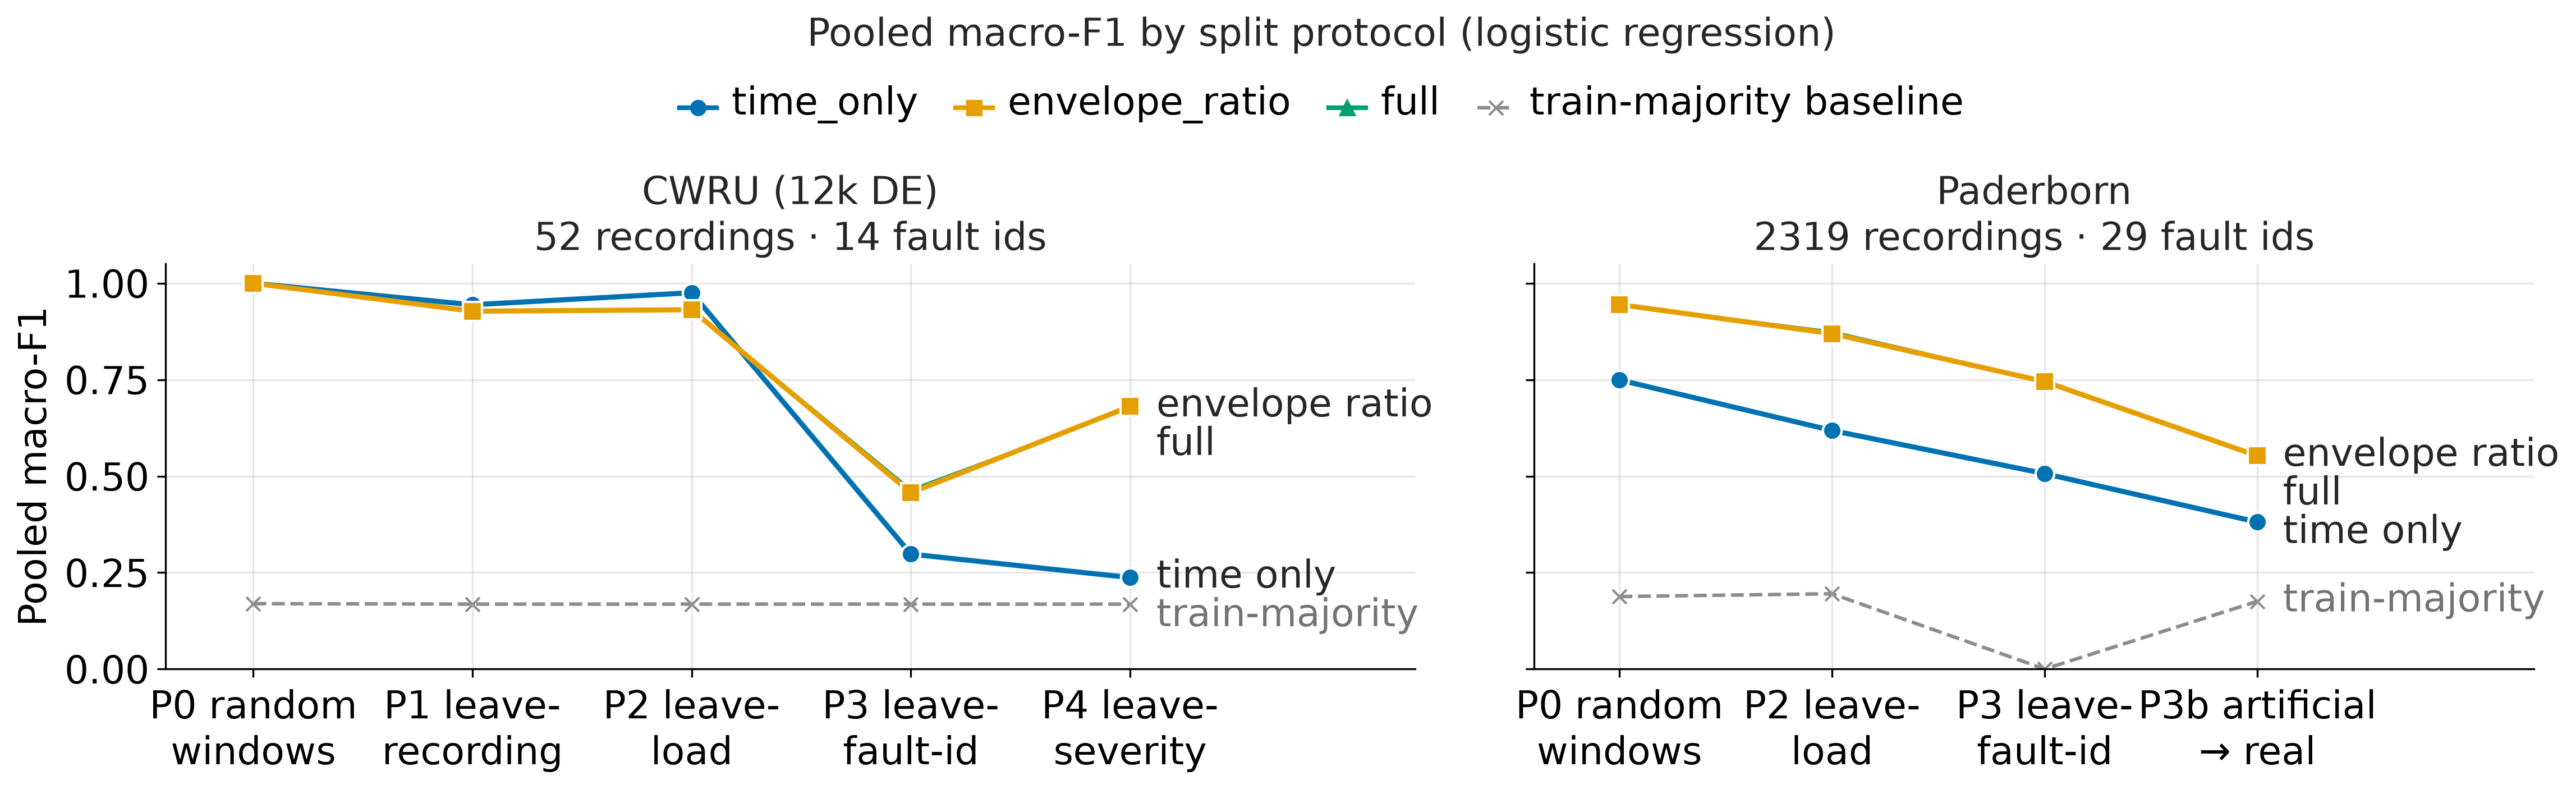
\includegraphics[width=\textwidth]{figures/C1_ladder_real.png}}
\caption{Pooled macro-F1 by split protocol for each feature set on CWRU (left) and Paderborn (right), logistic
regression, measured shaft speed. The dashed line is the train-majority baseline.}
\label{fig:ladder}
\end{figure*}

\begin{table}[t]
\caption{Pooled macro-F1 along the split ladder (logistic regression, measured shaft speed). Env.\ = envelope\_ratio, Time = time\_only; -- = protocol not applicable to the dataset.}
\label{tab:ladder}
\centering
\setlength{\tabcolsep}{4pt}
\begin{tabular}{lcccc}
\hline
 & \multicolumn{2}{c}{CWRU} & \multicolumn{2}{c}{Paderborn} \\
Protocol & Env. & Time & Env. & Time \\
\hline
P0 random windows & 1.000 & 1.000 & 0.945 & 0.749 \\
P1 leave-one-recording-out & 0.928 & 0.944 & -- & -- \\
P2 leave-one-load-out & 0.931 & 0.975 & 0.869 & 0.618 \\
P3 leave-one-fault-out & 0.457 & 0.298 & 0.745 & 0.506 \\
P3b artificial $\rightarrow$ real & -- & -- & 0.553 & 0.381 \\
P4 leave-one-severity-out & 0.681 & 0.237 & -- & -- \\
\hline
\end{tabular}
\end{table}


\subsection{Envelope versus time-domain features}

Table~\ref{tab:headline} reports the honest splits with confidence intervals. With logistic regression, envelope
features gain \val{paderborn-logreg-P3-diff} on Paderborn P3, \val{paderborn-logreg-P3b-diff} when training on
artificial and testing on real damage, and \val{cwru-logreg-P4-diff} on CWRU P4. On CWRU P3 the gain
(\val{cwru-logreg-P3-diff}) is not significant with only \val{cwru-ids} faults. GBDT shows the same collapse from random to honest splits (Figure~\ref{fig:ladder-gbdt}) and confirms the
CWRU P4 and Paderborn P3b gains. On Paderborn P3 it extracts more from the time-domain features, and the gap narrows to
\val{paderborn-gbdt-P3-diff}. Across \val{seed-n} GBDT seeds, P3 macro-F1 moves by at most \val{seed-maxsd} (standard
deviation).

\begin{table*}[t]
\caption{Pooled macro-F1 on the honest splits with 95\% fault-level bootstrap intervals, measured shaft speed. $\Delta$ is envelope\_ratio minus time\_only from a paired bootstrap; $^{*}$ marks intervals that exclude zero.}
\label{tab:headline}
\centering
\begin{tabular}{llccc}
\hline
Split & Model & envelope\_ratio & time\_only & $\Delta$ (95\% CI) \\
\hline
CWRU, P3 & LR & 0.457 [0.25, 0.75] & 0.298 [0.15, 0.53] & +0.16 [$-$0.06, +0.40] \\
CWRU, P4 & LR & 0.681 [0.46, 0.84] & 0.237 [0.08, 0.34] & +0.44 [+0.28, +0.61]$^{*}$ \\
Paderborn, P3 & LR & 0.745 [0.58, 0.86] & 0.506 [0.37, 0.61] & +0.24 [+0.15, +0.33]$^{*}$ \\
Paderborn, P3b & LR & 0.553 [0.31, 0.78] & 0.381 [0.15, 0.57] & +0.17 [+0.06, +0.30]$^{*}$ \\
CWRU, P3 & GBDT & 0.505 [0.25, 0.85] & 0.311 [0.15, 0.55] & +0.19 [$-$0.09, +0.47] \\
CWRU, P4 & GBDT & 0.748 [0.48, 0.91] & 0.432 [0.13, 0.55] & +0.32 [+0.10, +0.61]$^{*}$ \\
Paderborn, P3 & GBDT & 0.700 [0.55, 0.81] & 0.657 [0.51, 0.77] & +0.04 [$-$0.04, +0.11] \\
Paderborn, P3b & GBDT & 0.587 [0.35, 0.81] & 0.388 [0.19, 0.58] & +0.20 [+0.08, +0.35]$^{*}$ \\
\hline
\end{tabular}
\end{table*}


\begin{figure*}[t]
\centerline{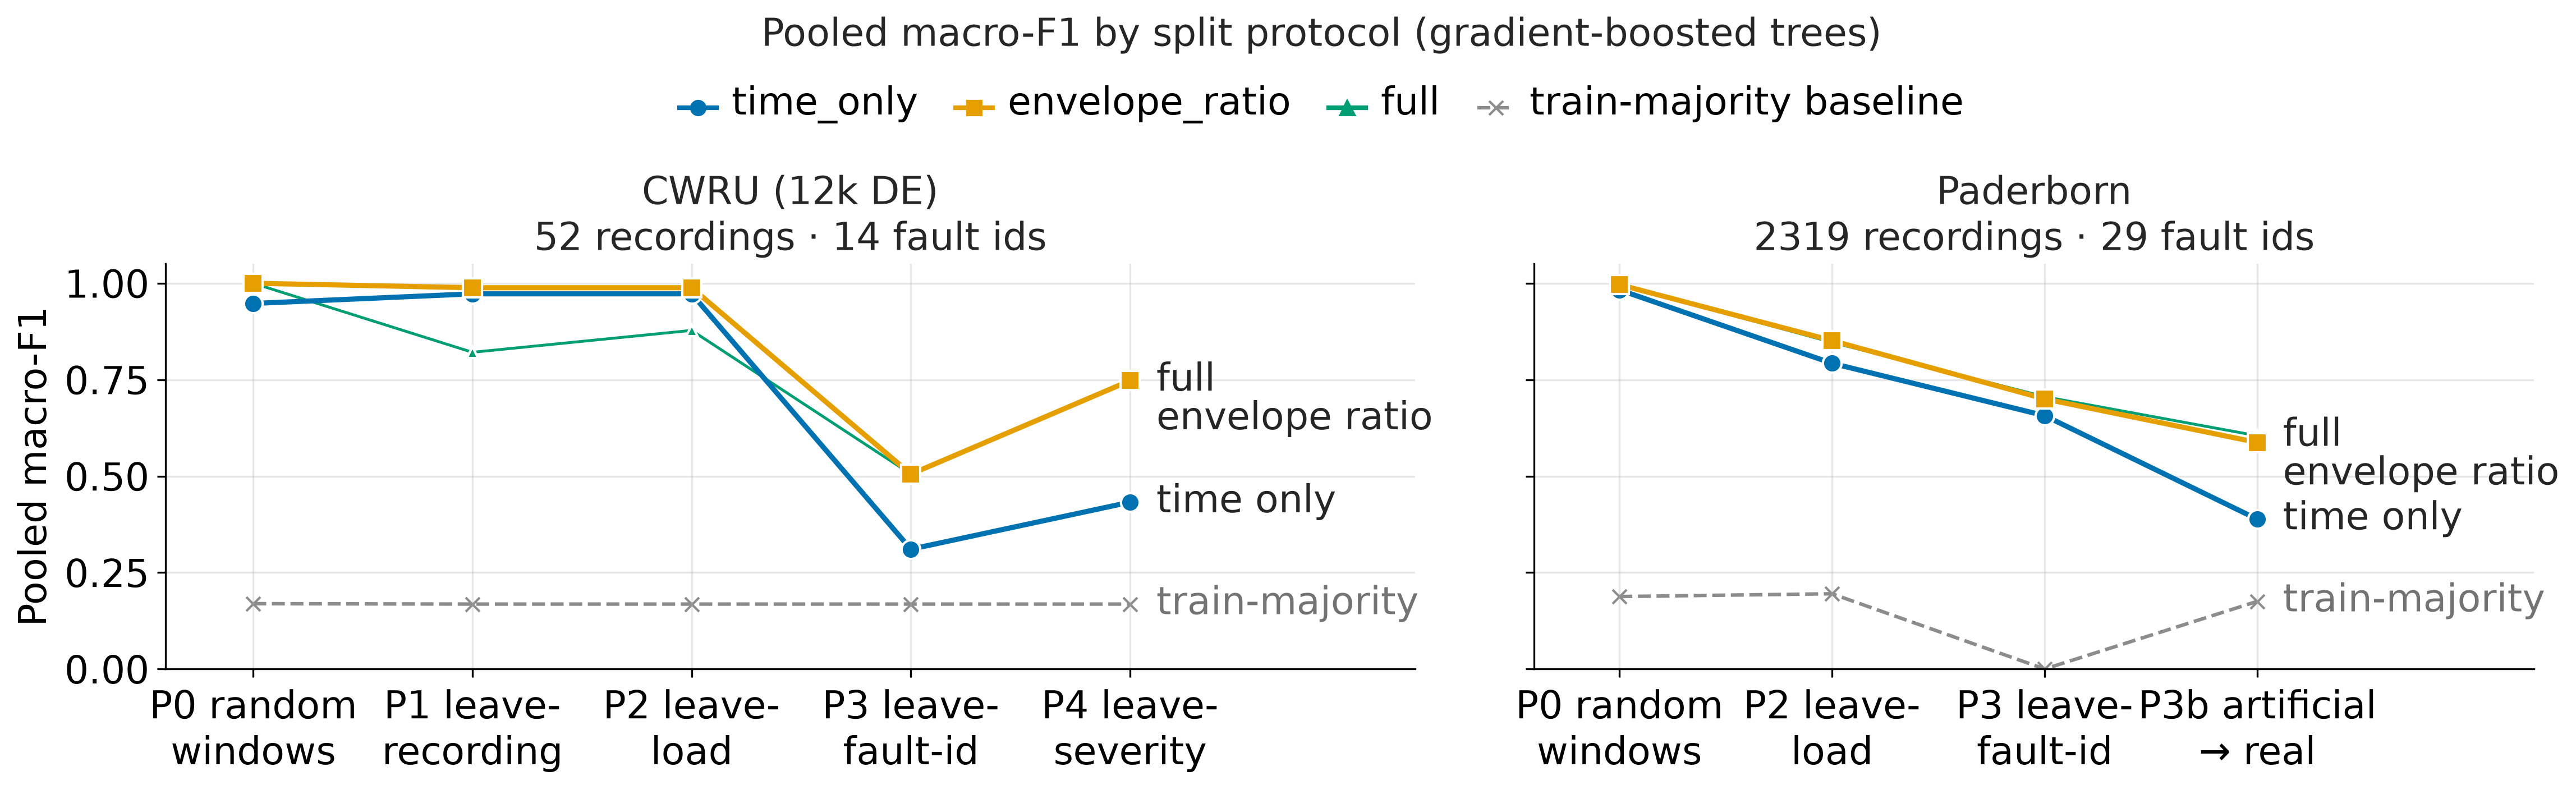
\includegraphics[width=\textwidth]{figures/C1_ladder_real_gbdt.png}}
\caption{Pooled macro-F1 by split protocol with gradient-boosted trees: the same collapse from random windows to
held-out faults as with logistic regression (Figure~\ref{fig:ladder}).}
\label{fig:ladder-gbdt}
\end{figure*}

CWRU's single healthy bearing makes healthy F1 zero under P3 by construction, because its fold trains with no
healthy data. Averaged over the three fault classes only, CWRU P3 scores \val{cwru-logreg-P3-env-xh}
\val{cwru-logreg-P3-env-xhci} with envelope features and \val{cwru-logreg-P3-time-xh} with time-domain features.
Figure~\ref{fig:confusion} shows where the errors fall. Figure~\ref{fig:folds} shows that envelope features
classify most held-out outer- and inner-race faults correctly, while ball faults remain partial.

\begin{figure}[t]
\centerline{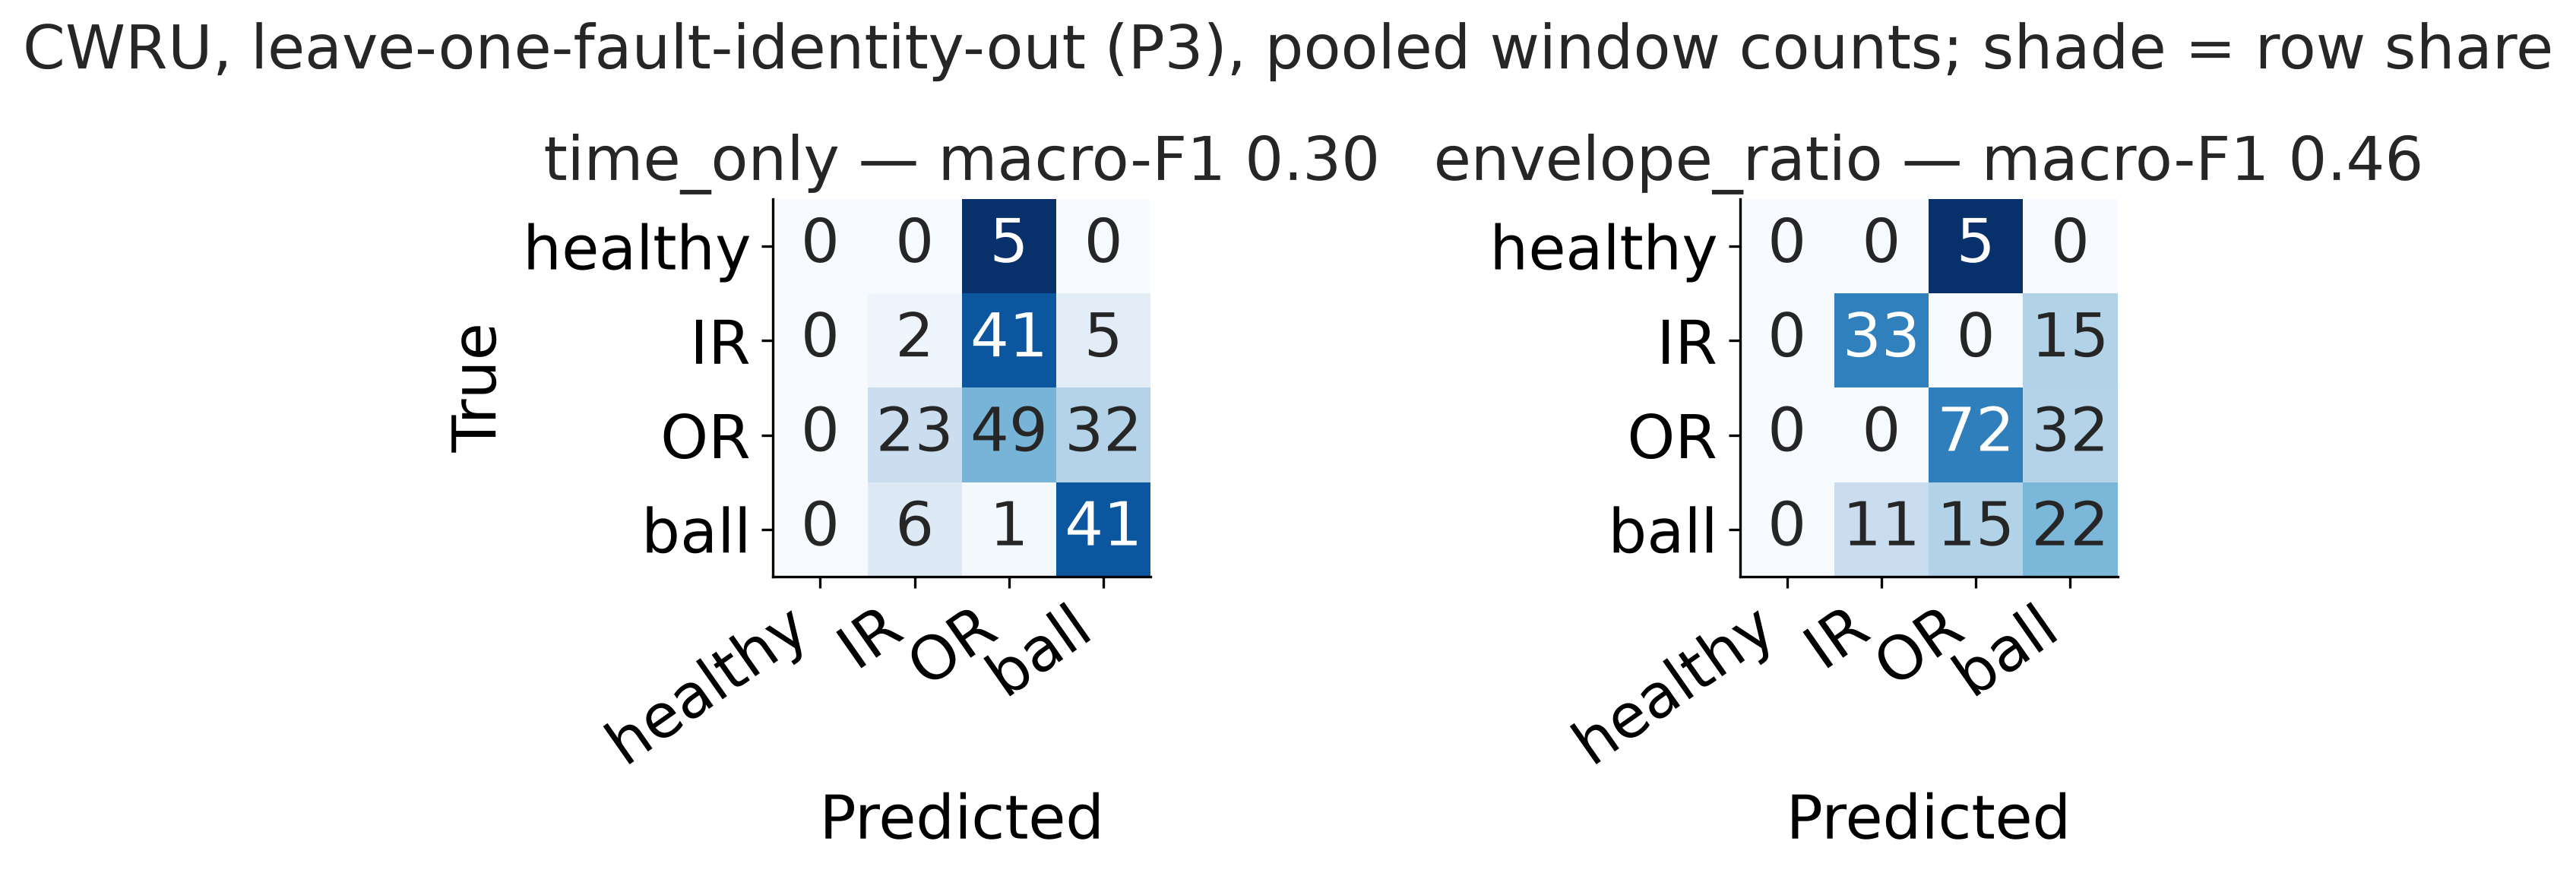
\includegraphics[width=\columnwidth]{figures/C2_confusion_cwru_P3.png}}
\caption{Pooled confusion matrices on CWRU P3 (leave-one-fault-out) for time\_only (left) and envelope\_ratio
(right); counts are windows, and shading is the share of each true class.}
\label{fig:confusion}
\end{figure}

\begin{figure}[t]
\centerline{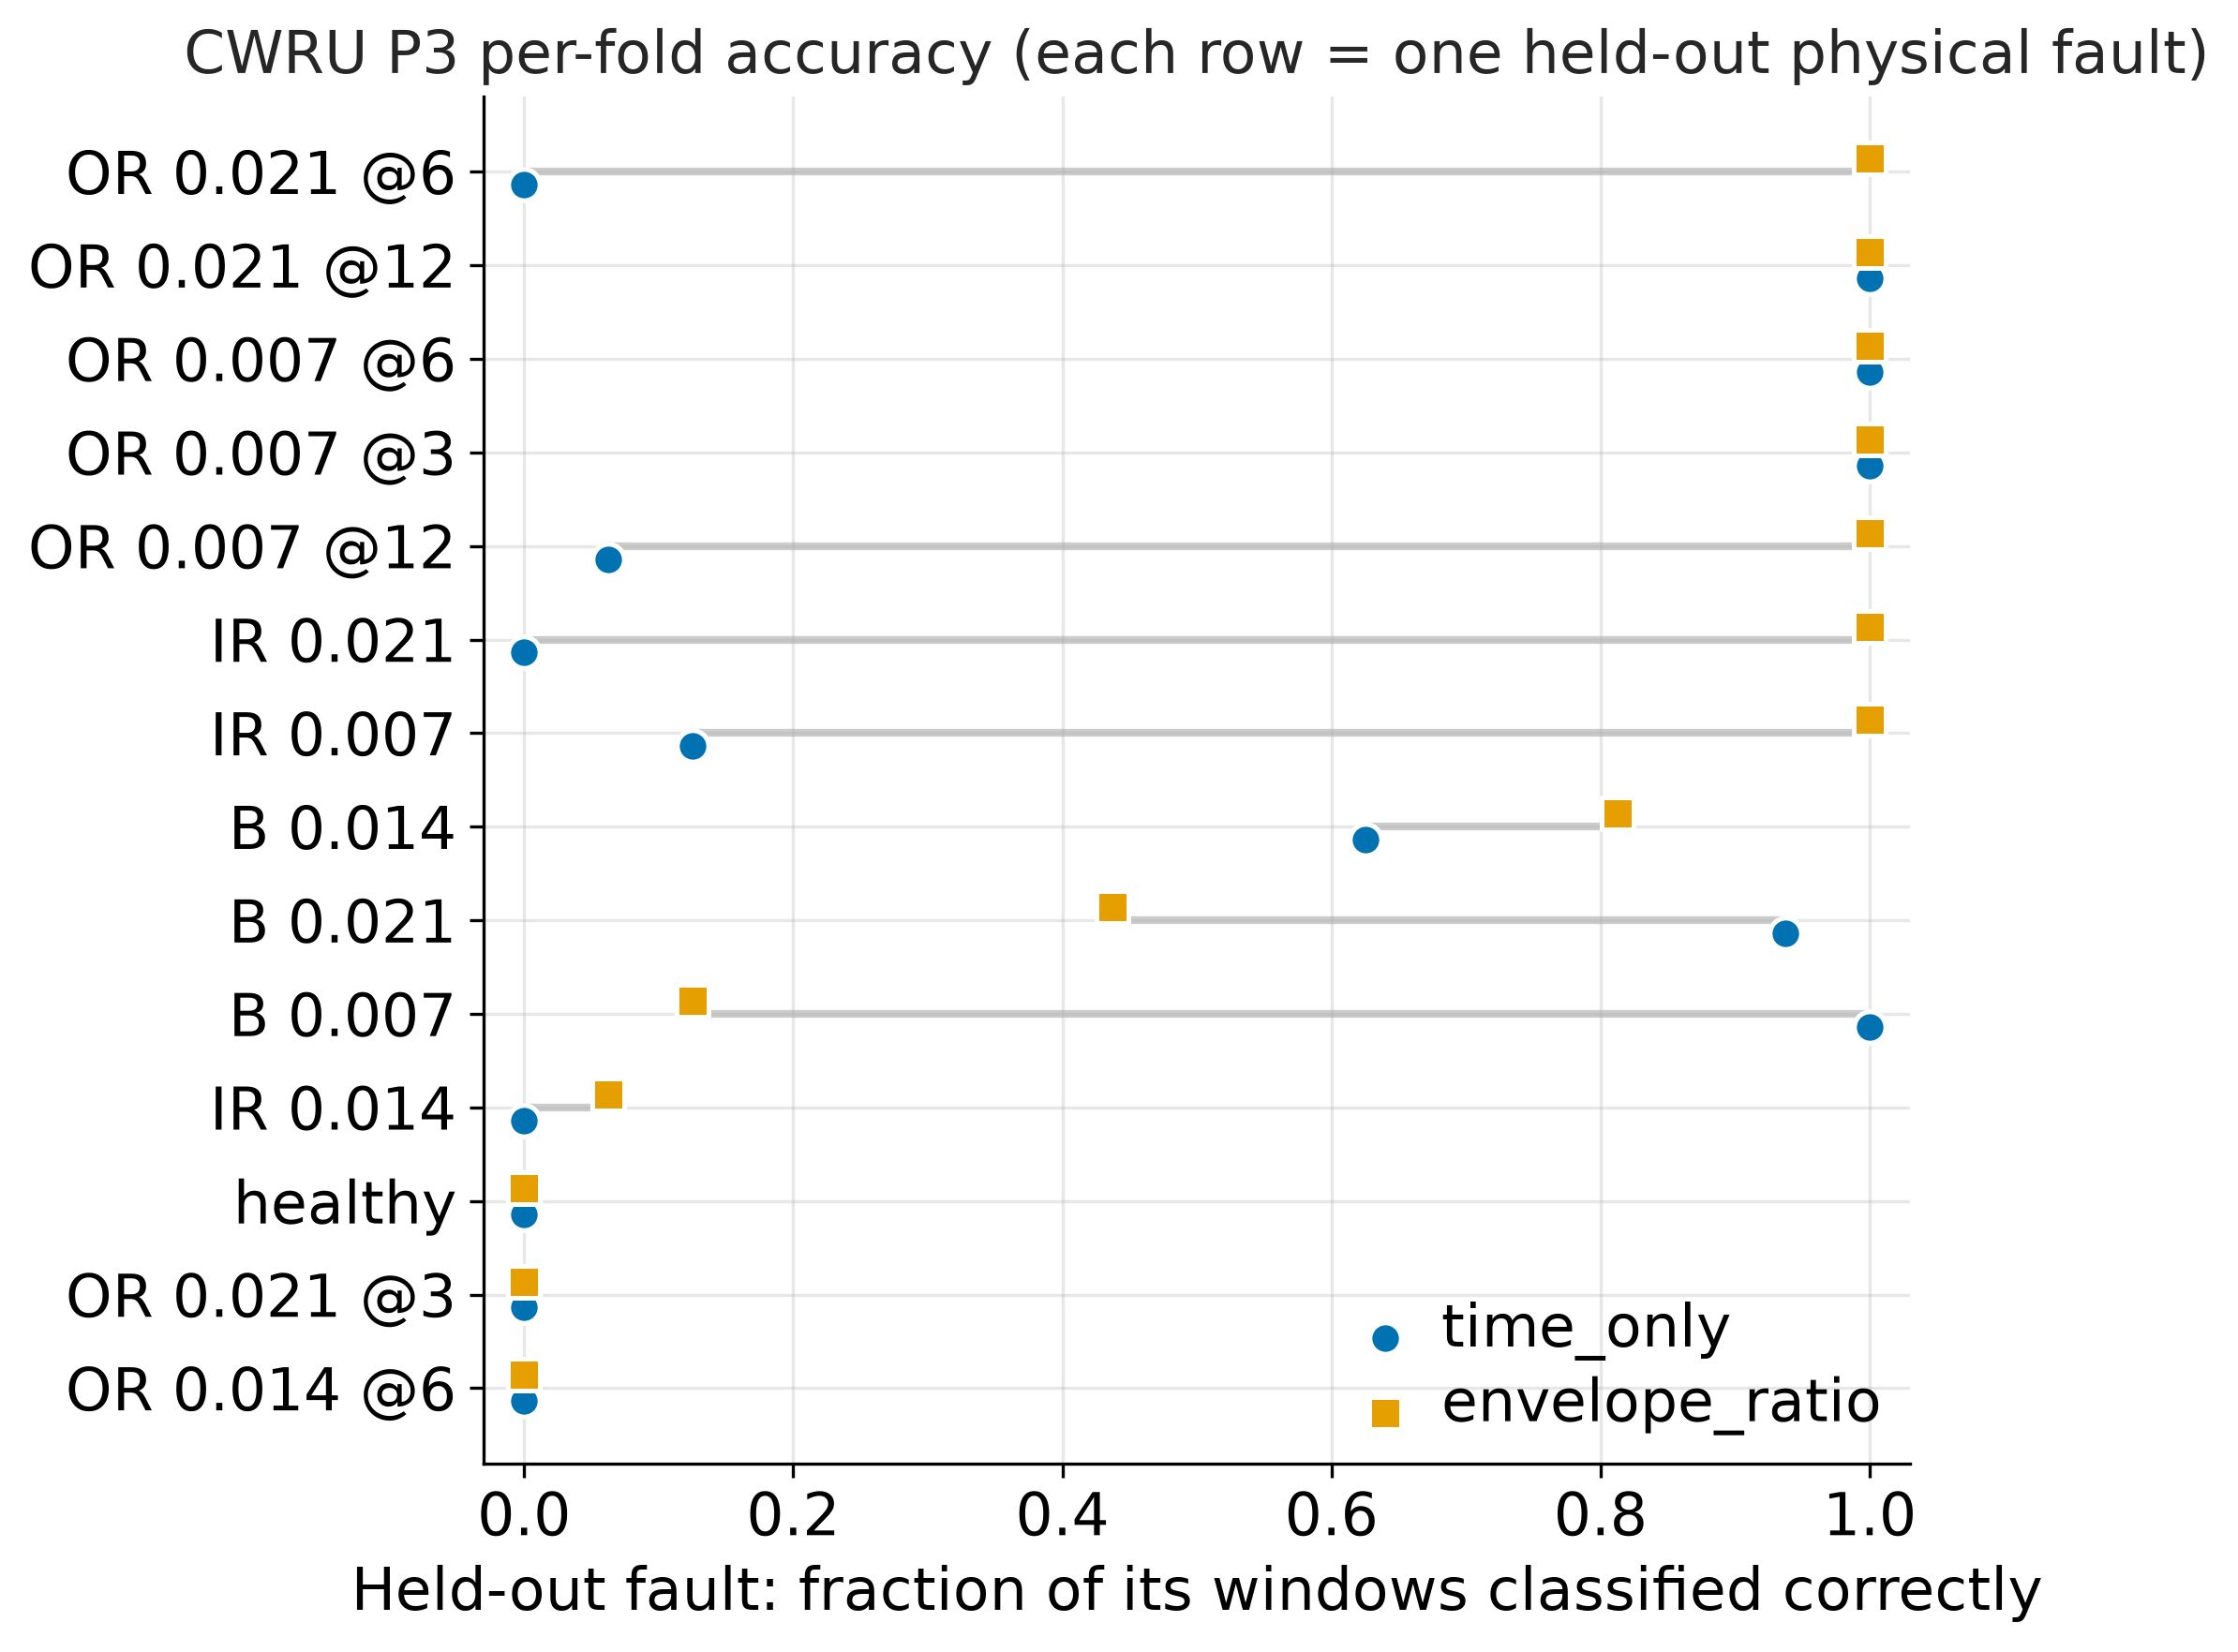
\includegraphics[width=\columnwidth]{figures/C6_fold_spread_cwru_P3.png}}
\caption{Per-fold accuracy on CWRU P3: each row is one held-out physical fault.}
\label{fig:folds}
\end{figure}

\subsection{Overfitting to fault identity}

Figure~\ref{fig:loss} shows GBDT log-loss after each of \val{lc-cwru-nest} boosting stages. Under random windows,
held-out loss keeps falling and held-out macro-F1 reaches \val{lc-paderborn-env-p0f1} on Paderborn. Under
leave-one-fault-out, held-out loss is lowest after \val{lc-cwru-env-best} (CWRU) and \val{lc-paderborn-env-best}
(Paderborn) stages, then rises while training loss approaches zero. The additional trees therefore memorise the
training faults rather than the fault types. The stage of minimum loss is chosen on the held-out data, so it is
descriptive, not a tuned stopping point.

\begin{figure*}[t]
\centerline{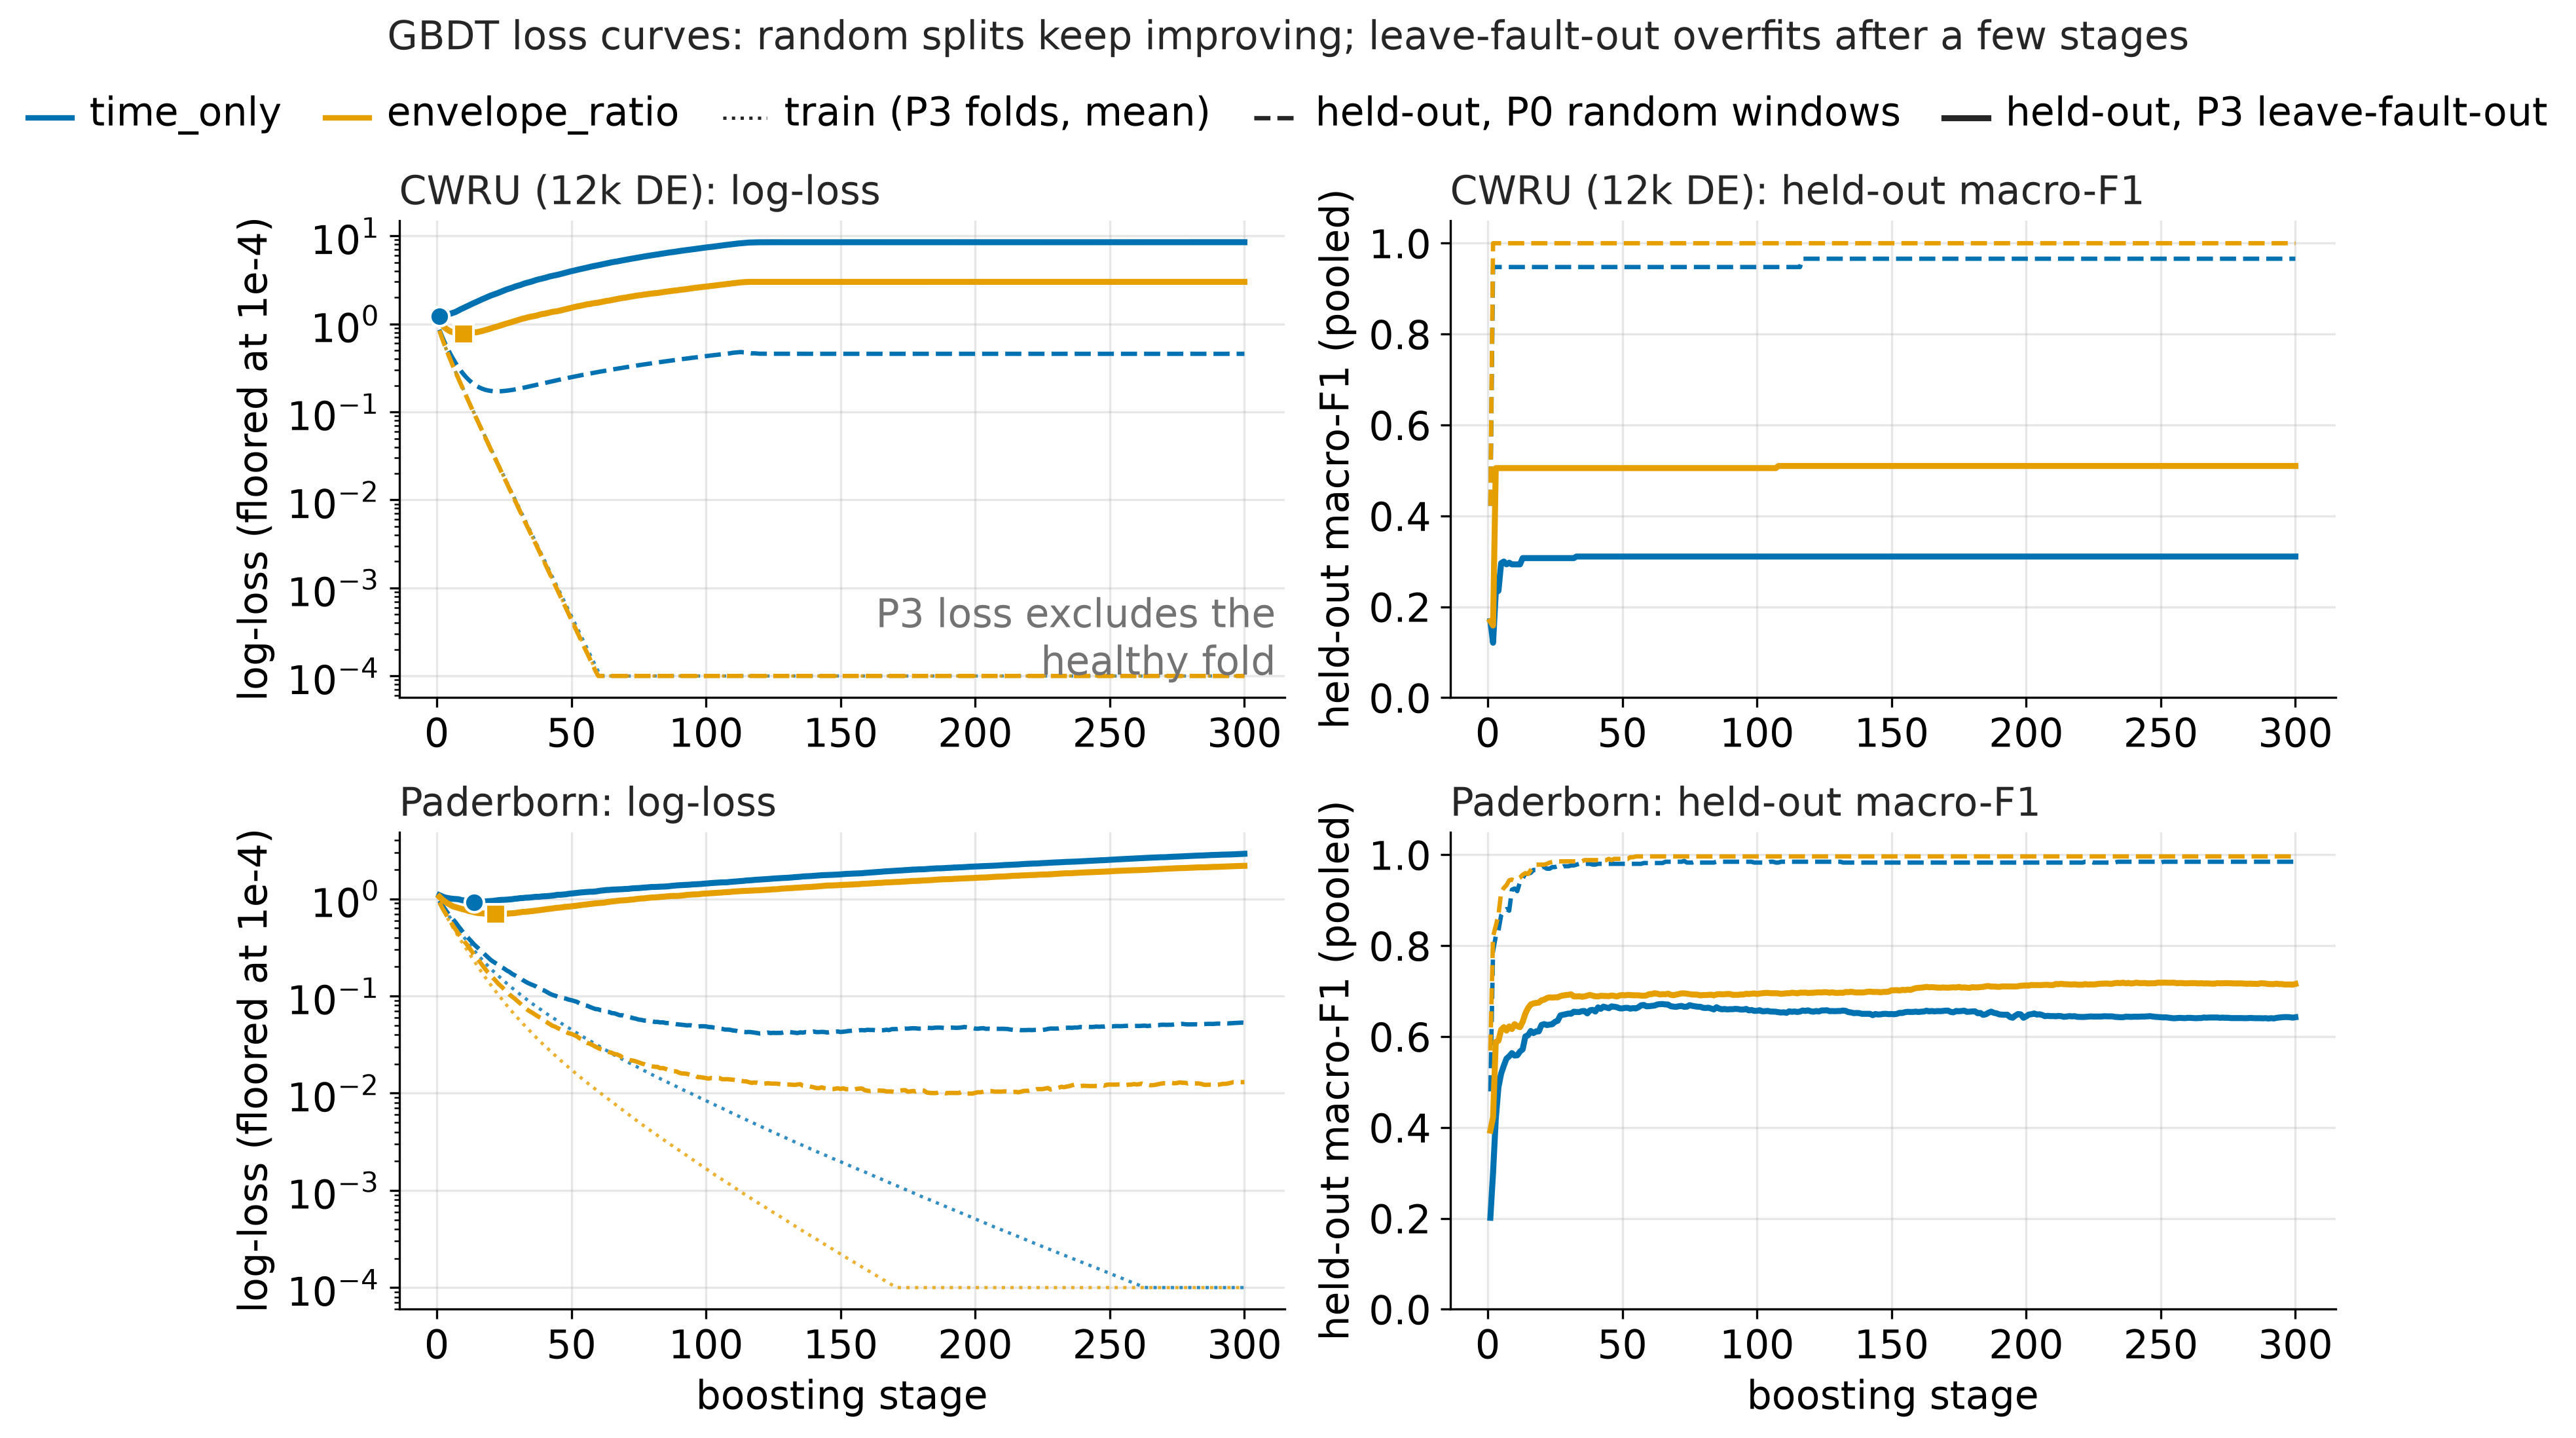
\includegraphics[width=0.8\textwidth]{figures/loss_curves_gbdt.png}}
\caption{GBDT training and held-out log-loss (left) and held-out macro-F1 (right) per boosting stage, for random
windows (P0, dashed) and leave-one-fault-out (P3, solid), CWRU (top) and Paderborn (bottom).}
\label{fig:loss}
\end{figure*}

\subsection{Transfer and severity}

Across datasets (Figure~\ref{fig:transfer}), a model trained on Paderborn with envelope features transfers to MFPT
(\val{tr-env-paderborn-mfpt}) and CWRU (\val{tr-env-paderborn-cwru}). The time-only model reaches at most
\val{tr-time-offmax} off its own dataset. On MaFaulDa, imbalance remains detectable at held-out masses for every
feature set: \val{sev-interp-env} (envelope) and \val{sev-interp-time} (time) when interpolating, against a baseline
of \val{sev-interp-base}. That task is easy enough that it does not separate the feature sets (Figure~\ref{fig:severity}).

\begin{figure}[t]
\centerline{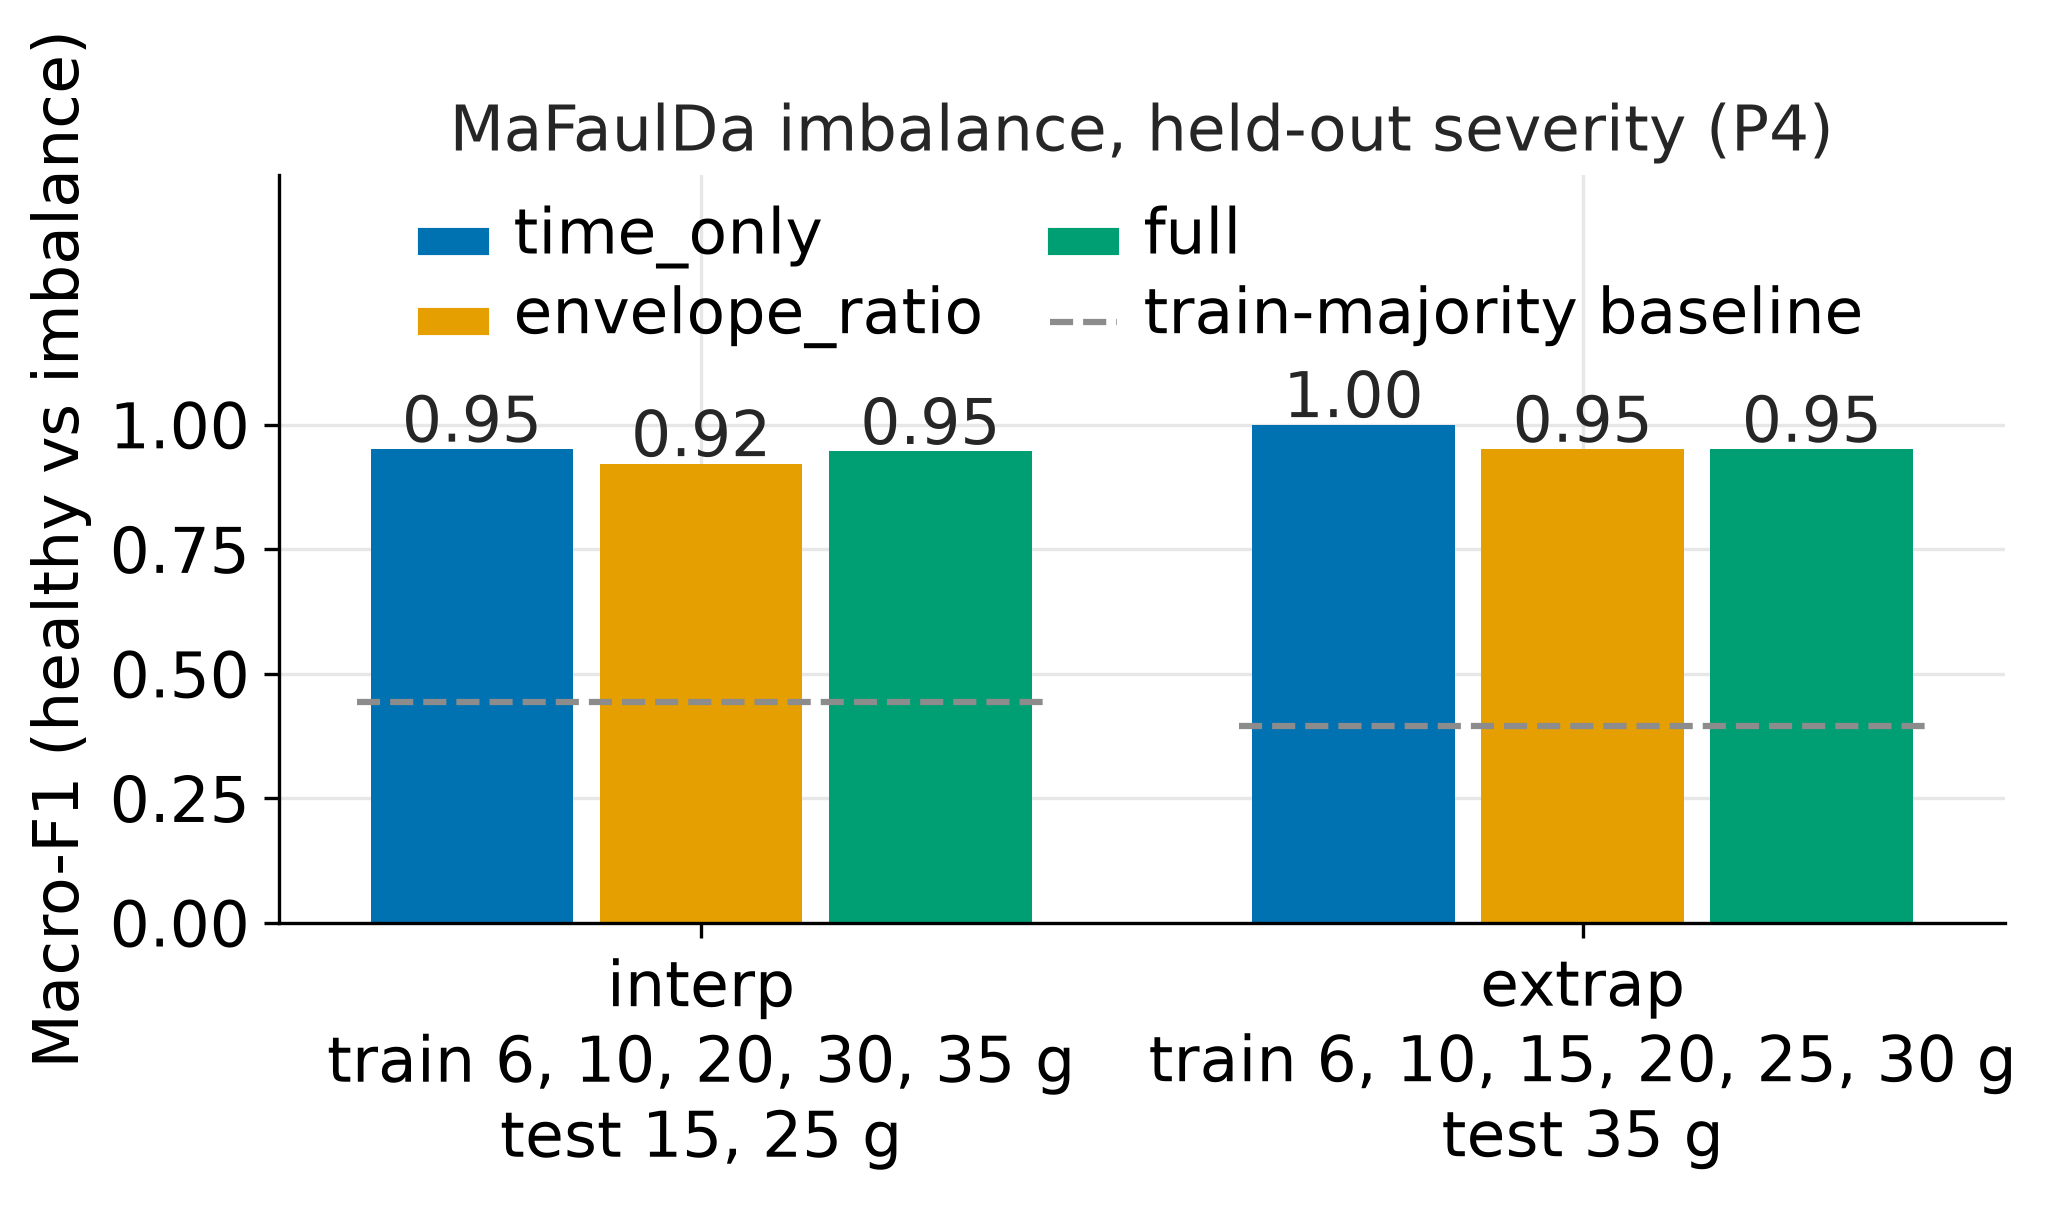
\includegraphics[width=\columnwidth]{figures/C11_severity_mafaulda.png}}
\caption{MaFaulDa healthy-versus-imbalance macro-F1 when the imbalance mass is held out: interpolation (train
6--35~g without 15 and 25~g, test 15 and 25~g) and extrapolation (test 35~g). The dashed lines are the
train-majority baseline.}
\label{fig:severity}
\end{figure}

\begin{figure}[t]
\centerline{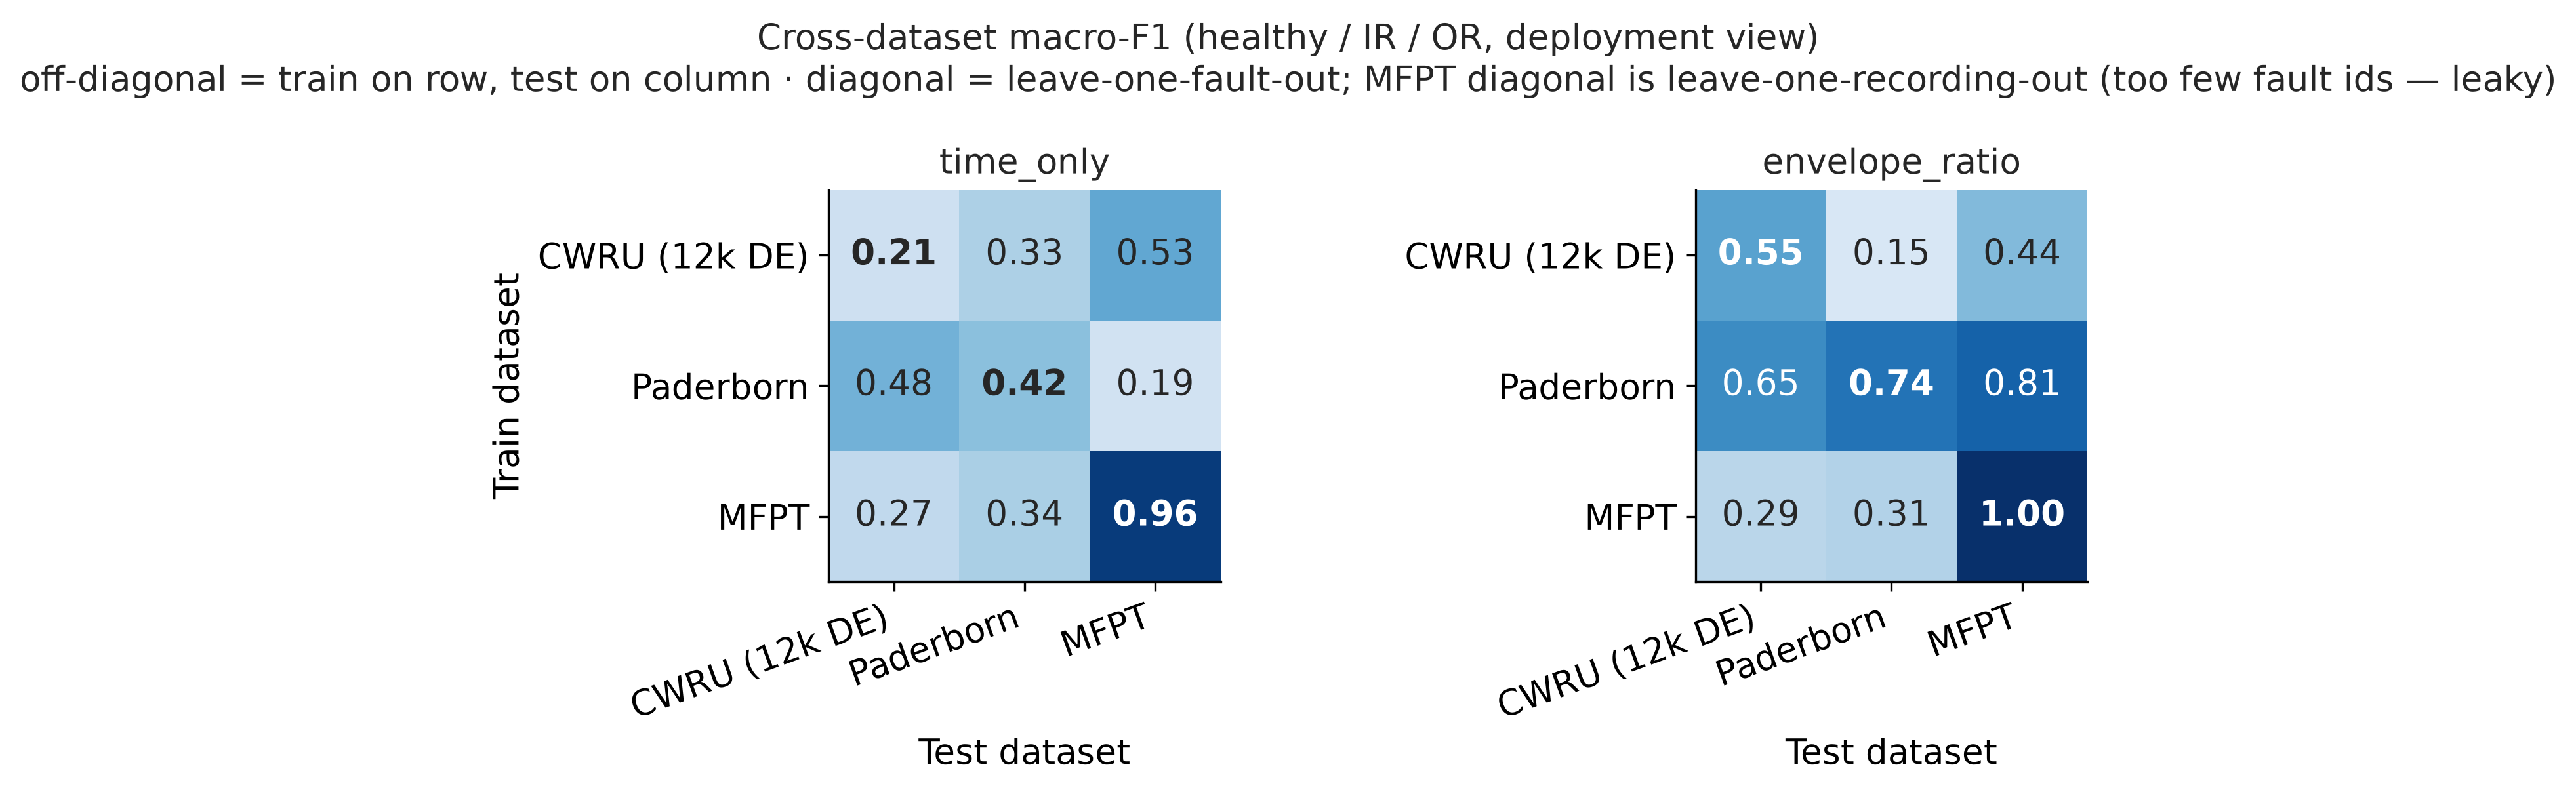
\includegraphics[width=\columnwidth]{figures/C10_transfer_real.png}}
\caption{Cross-dataset macro-F1 (train on row, test on column; classes healthy, inner race, outer race) for
time\_only (left) and envelope\_ratio (right). The diagonal is within-dataset leave-one-fault-out; the MFPT diagonal
uses leave-one-recording-out and is inflated.}
\label{fig:transfer}
\end{figure}

\subsection{Physical check}

Figure~\ref{fig:envelope} shows real CWRU envelope spectra with the kinematic frequencies of~\eqref{eq:bpf}
marked. The inner-race fault peaks at BPFI and the outer-race fault at BPFO and its harmonics. The ball fault
produces only weak peaks, consistent with its partial classification in Figure~\ref{fig:folds}.

\begin{figure}[t]
\centerline{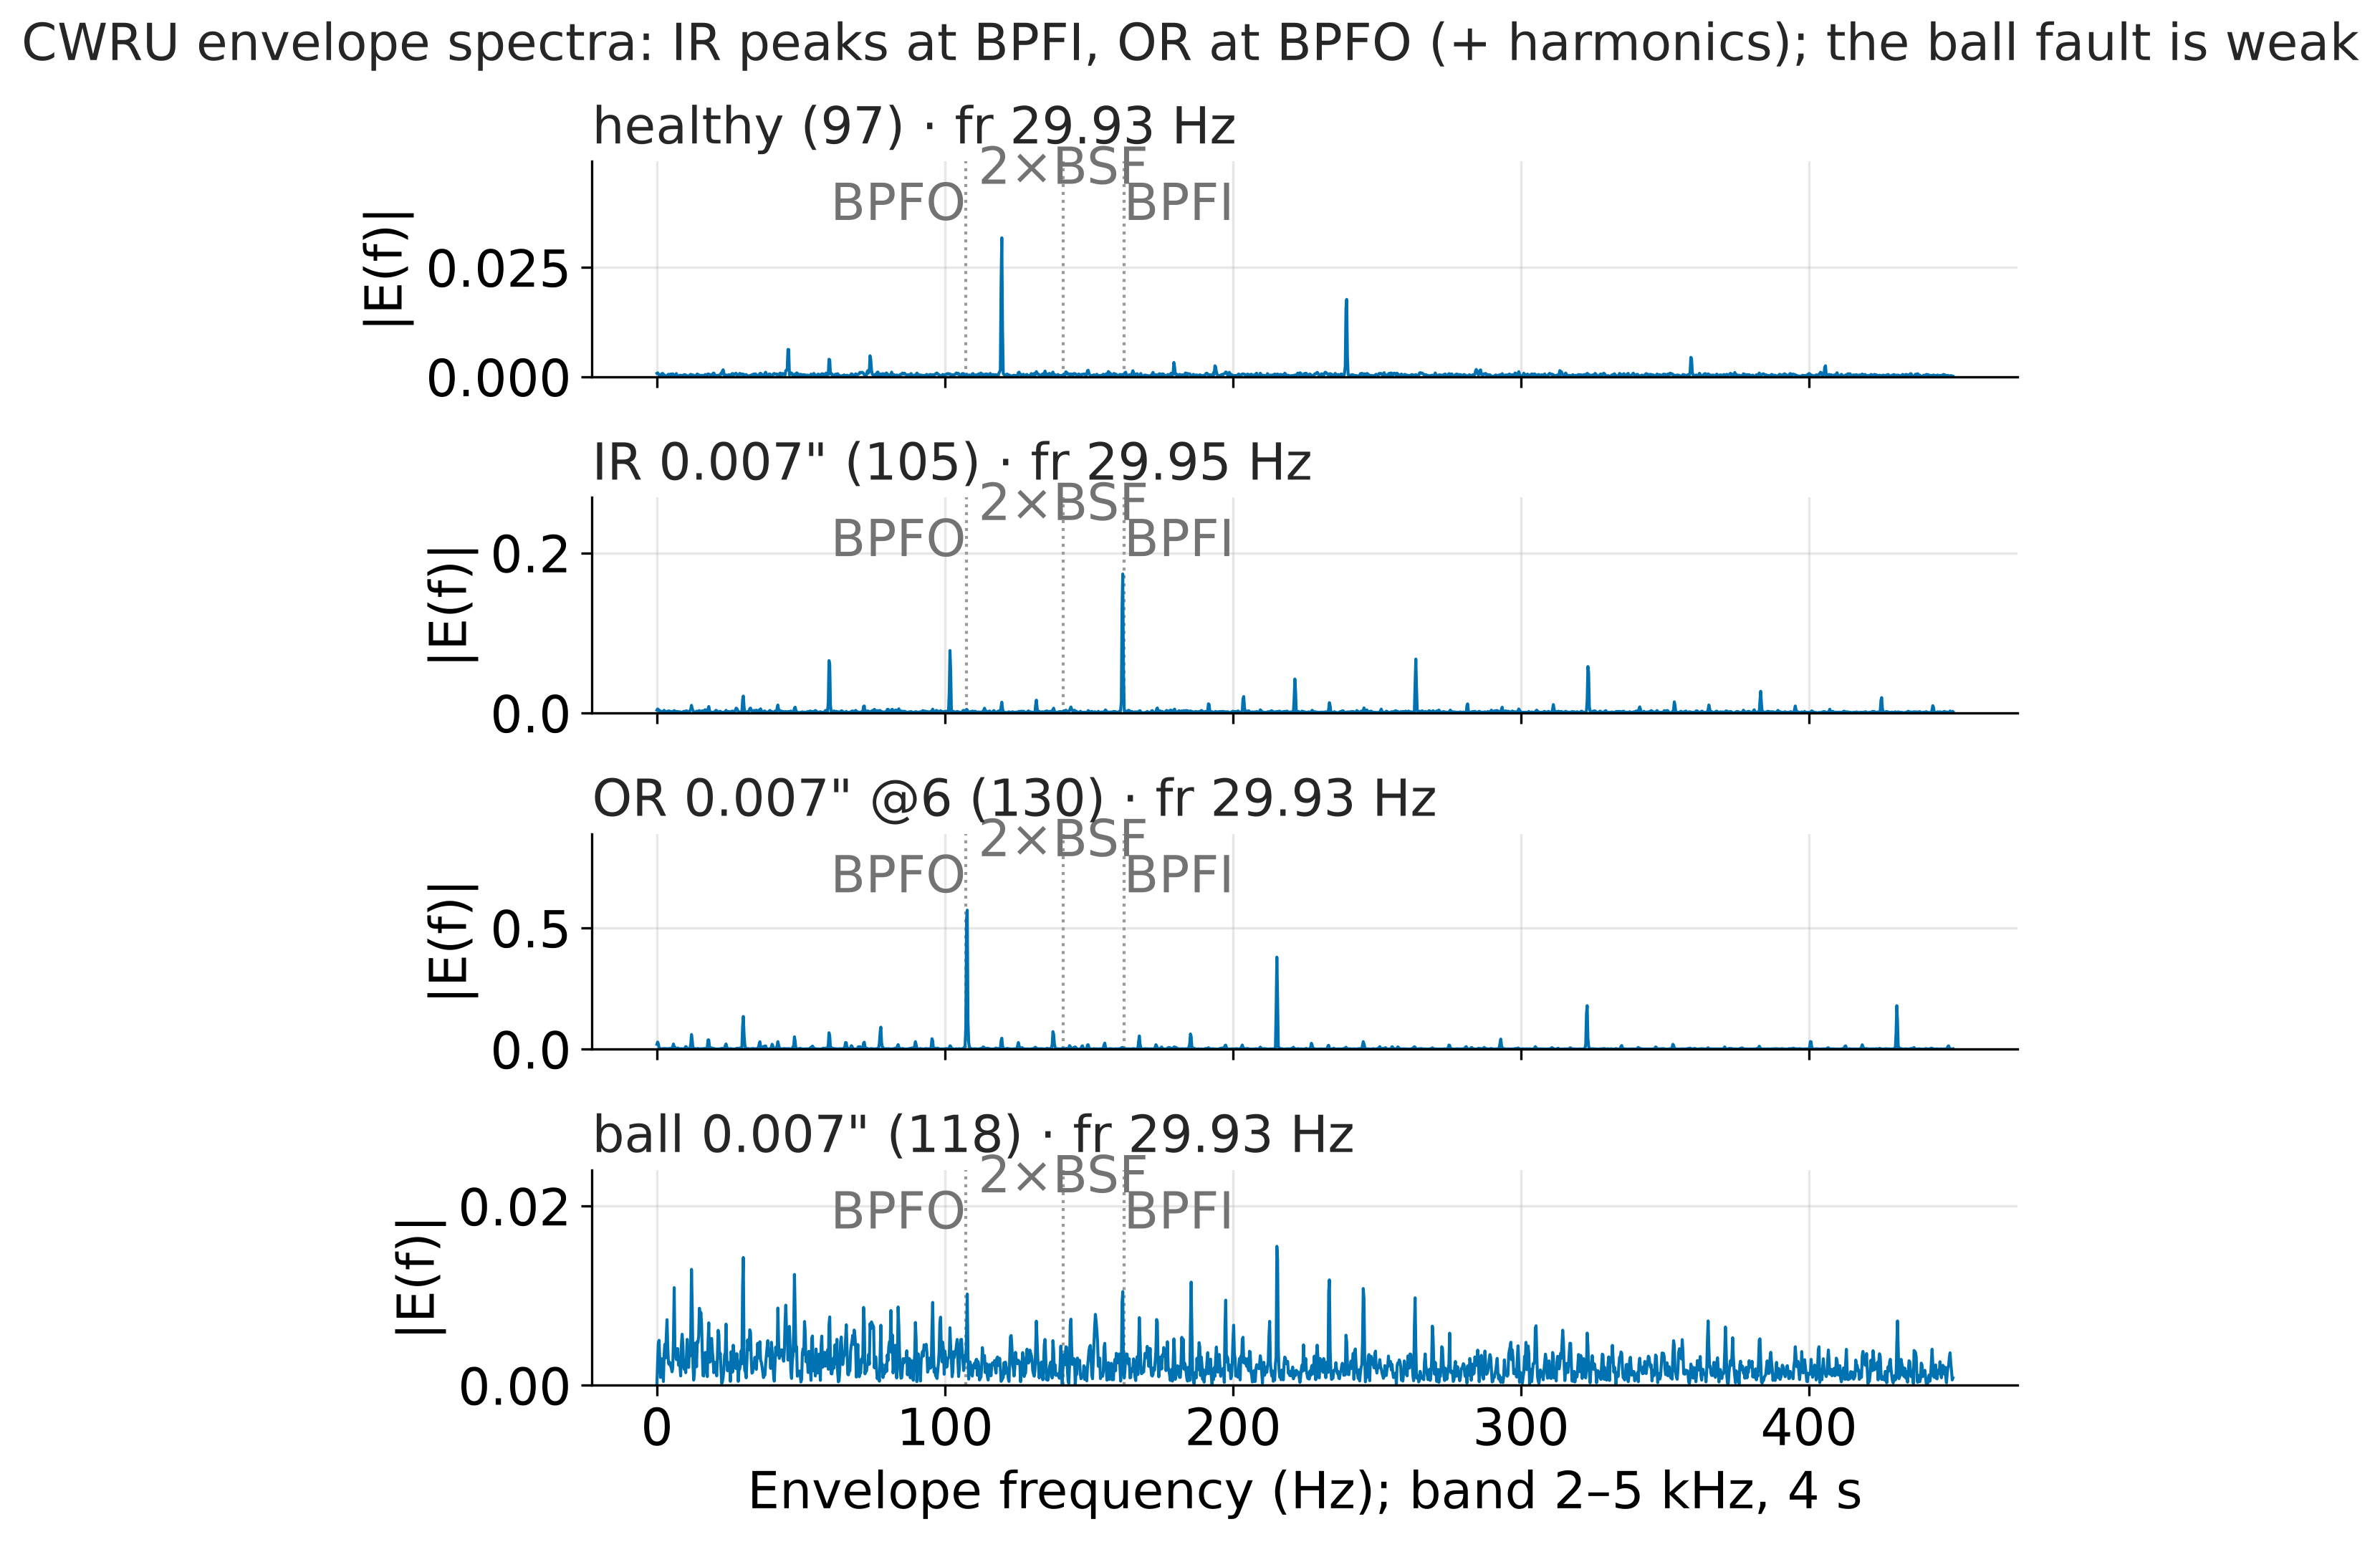
\includegraphics[width=\columnwidth]{figures/A3_envelope_cwru.png}}
\caption{Envelope spectra of CWRU recordings (healthy, inner race, outer race, ball) with BPFO, BPFI and
2$\times$BSF marked.}
\label{fig:envelope}
\end{figure}

% =====================================================================================================
\section{Shaft Speed: Measured versus Estimated}

Table~\ref{tab:speed} and Figure~\ref{fig:speed} show that the envelope advantage depends on the accuracy of the
shaft speed. On CWRU, the estimator restricted to the rated speed places \val{speed-cwru-prior-w2} of windows
within 2\% of the measured speed. With that prior, the gain equals the measured-speed gain (P4:
\val{speed-cwru-prior-P4-diff}). Over the generic 10--60~Hz range, it locks to twice the shaft rate on
\val{speed-cwru-estimated-2x} of windows. The likely cause is the 60~Hz mains line, which lies close to 2$\times$
the 29.95~Hz shaft rate.

On Paderborn the shaft line is weak. The estimator's confidence is usually low, so only
\val{speed-paderborn-estimated-used} of windows keep the speed-dependent features, and the gain shrinks to
\val{speed-paderborn-estimated-P3-diff}. The estimator was fixed against unit tests on synthetic signals; its
real-data accuracy was measured once, after those tests passed.

\begin{table*}[t]
\caption{Shaft-speed source versus envelope advantage (logistic regression). ``Within 2\%'' is the share of windows whose speed is within 2\% of the measured value; ``used'' is the share that keeps the speed-dependent features (the rest fall back to speed-free features); $\Delta$ as in Table~\ref{tab:headline}.}
\label{tab:speed}
\centering
\begin{tabular}{llcccl}
\hline
Dataset & Speed source & Within 2\% & Locked to 2$\times$ & Used & $\Delta$ envelope $-$ time (95\% CI) \\
\hline
CWRU & measured & 100\% & 0\% & 100\% & P3 +0.16 [$-$0.06, +0.40]; P4 +0.44 [+0.28, +0.61] \\
CWRU & estimated, rated $\pm$10\% & 100\% & 0\% & 100\% & P3 +0.16 [$-$0.06, +0.40]; P4 +0.45 [+0.29, +0.62] \\
CWRU & estimated, 10--60 Hz & 12\% & 67\% & 100\% & P3 +0.20 [$-$0.05, +0.43]; P4 +0.39 [+0.22, +0.68] \\
Paderborn & measured & 100\% & 0\% & 100\% & P3 +0.24 [+0.15, +0.33]; P3b +0.17 [+0.06, +0.30] \\
Paderborn & estimated, rated $\pm$10\% & 57\% & 0\% & 37\% & P3 +0.04 [$-$0.03, +0.11]; P3b $-$0.03 [$-$0.09, +0.02] \\
Paderborn & estimated, 10--60 Hz & 38\% & 12\% & 40\% & P3 +0.05 [$-$0.02, +0.12]; P3b +0.03 [$-$0.04, +0.09] \\
\hline
\end{tabular}
\end{table*}


\begin{figure*}[t]
\centerline{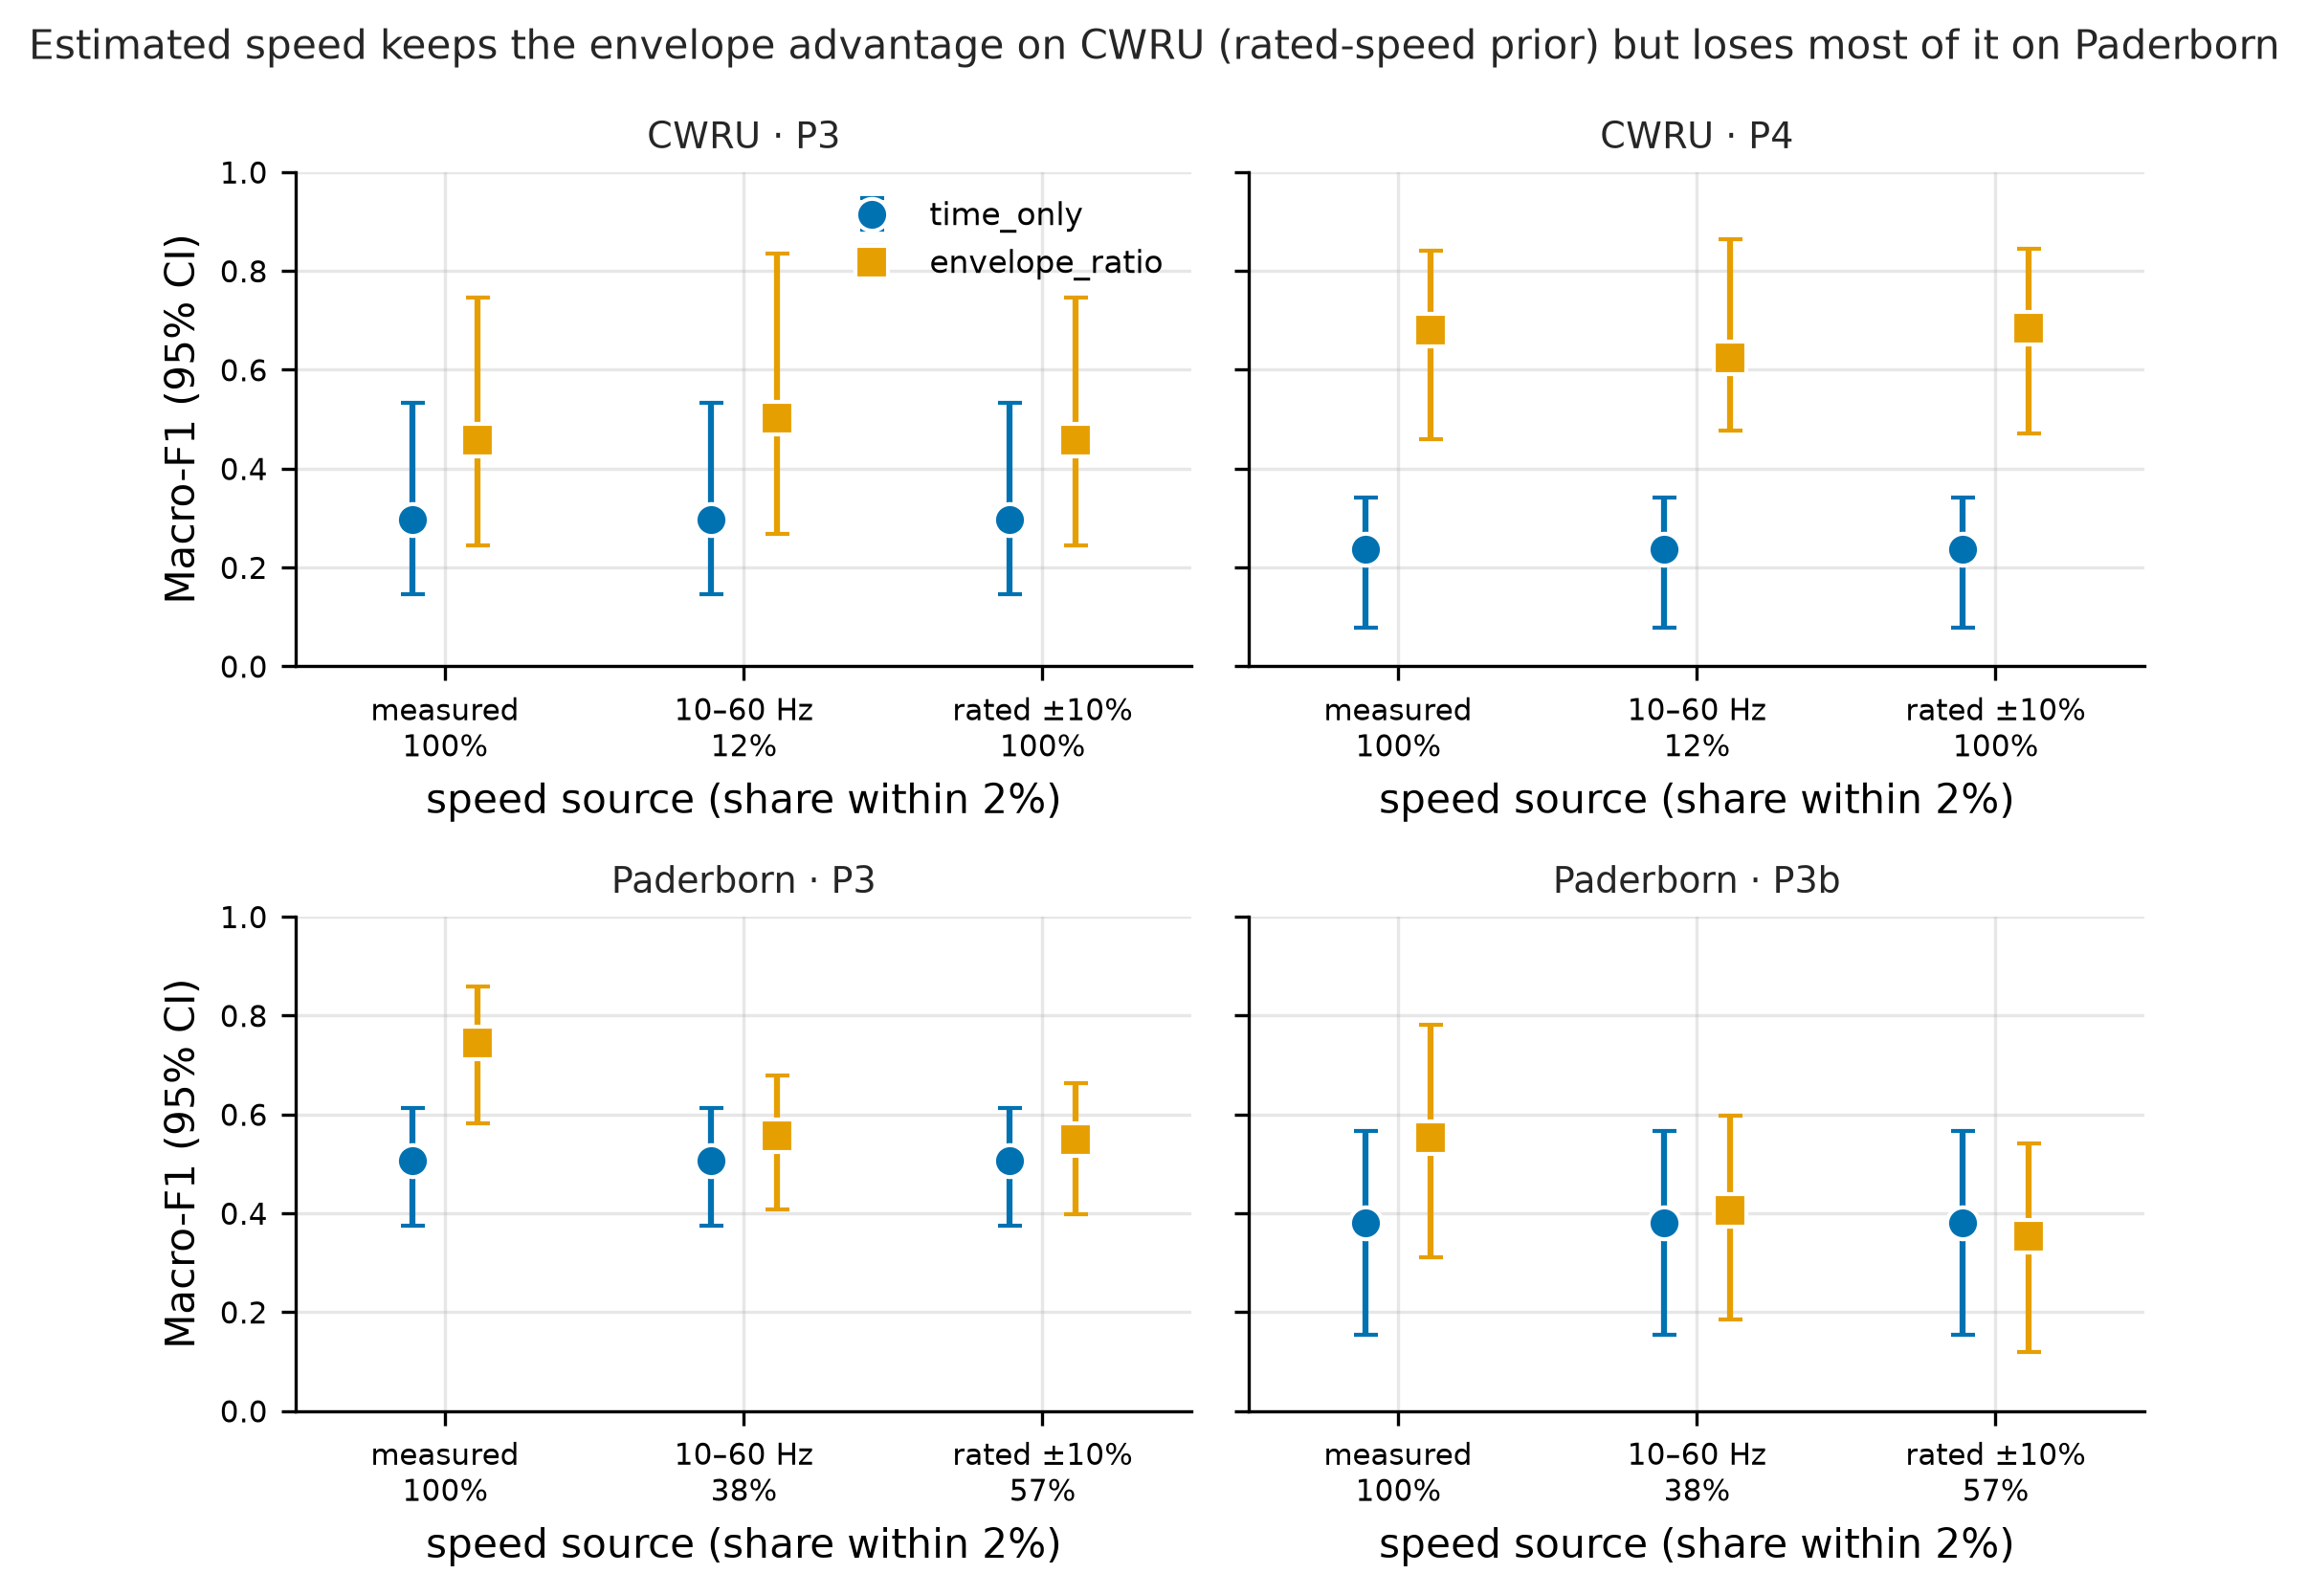
\includegraphics[width=\textwidth]{figures/speed_ablation.png}}
\caption{Honest-split macro-F1 with 95\% fault-level confidence intervals for measured speed, speed estimated over
10--60~Hz, and speed estimated within $\pm10\%$ of the rated speed.}
\label{fig:speed}
\end{figure*}

% =====================================================================================================
\section{Edge Deployment}

\subsection{Sensor view and cost}

We also pass each recording through a simulated low-cost sensor (Figure~\ref{fig:deploy}): a 6~kHz low-pass
filter, resampling to 26.7~kSPS, and MEMS accelerometer noise. On Paderborn P3 this lowers time\_only from
\val{dep-paderborn-pristine-time} to \val{dep-paderborn-deployment-time}, while envelope\_ratio holds
(\val{dep-paderborn-pristine-env} to \val{dep-paderborn-deployment-env}). Table~\ref{tab:cost} gives the model
cost. The envelope logistic regression needs \val{cost-envelope_ratio-params} parameters and a
\val{cost-envelope_ratio-bytes}-byte feature vector.

\begin{figure*}[t]
\centerline{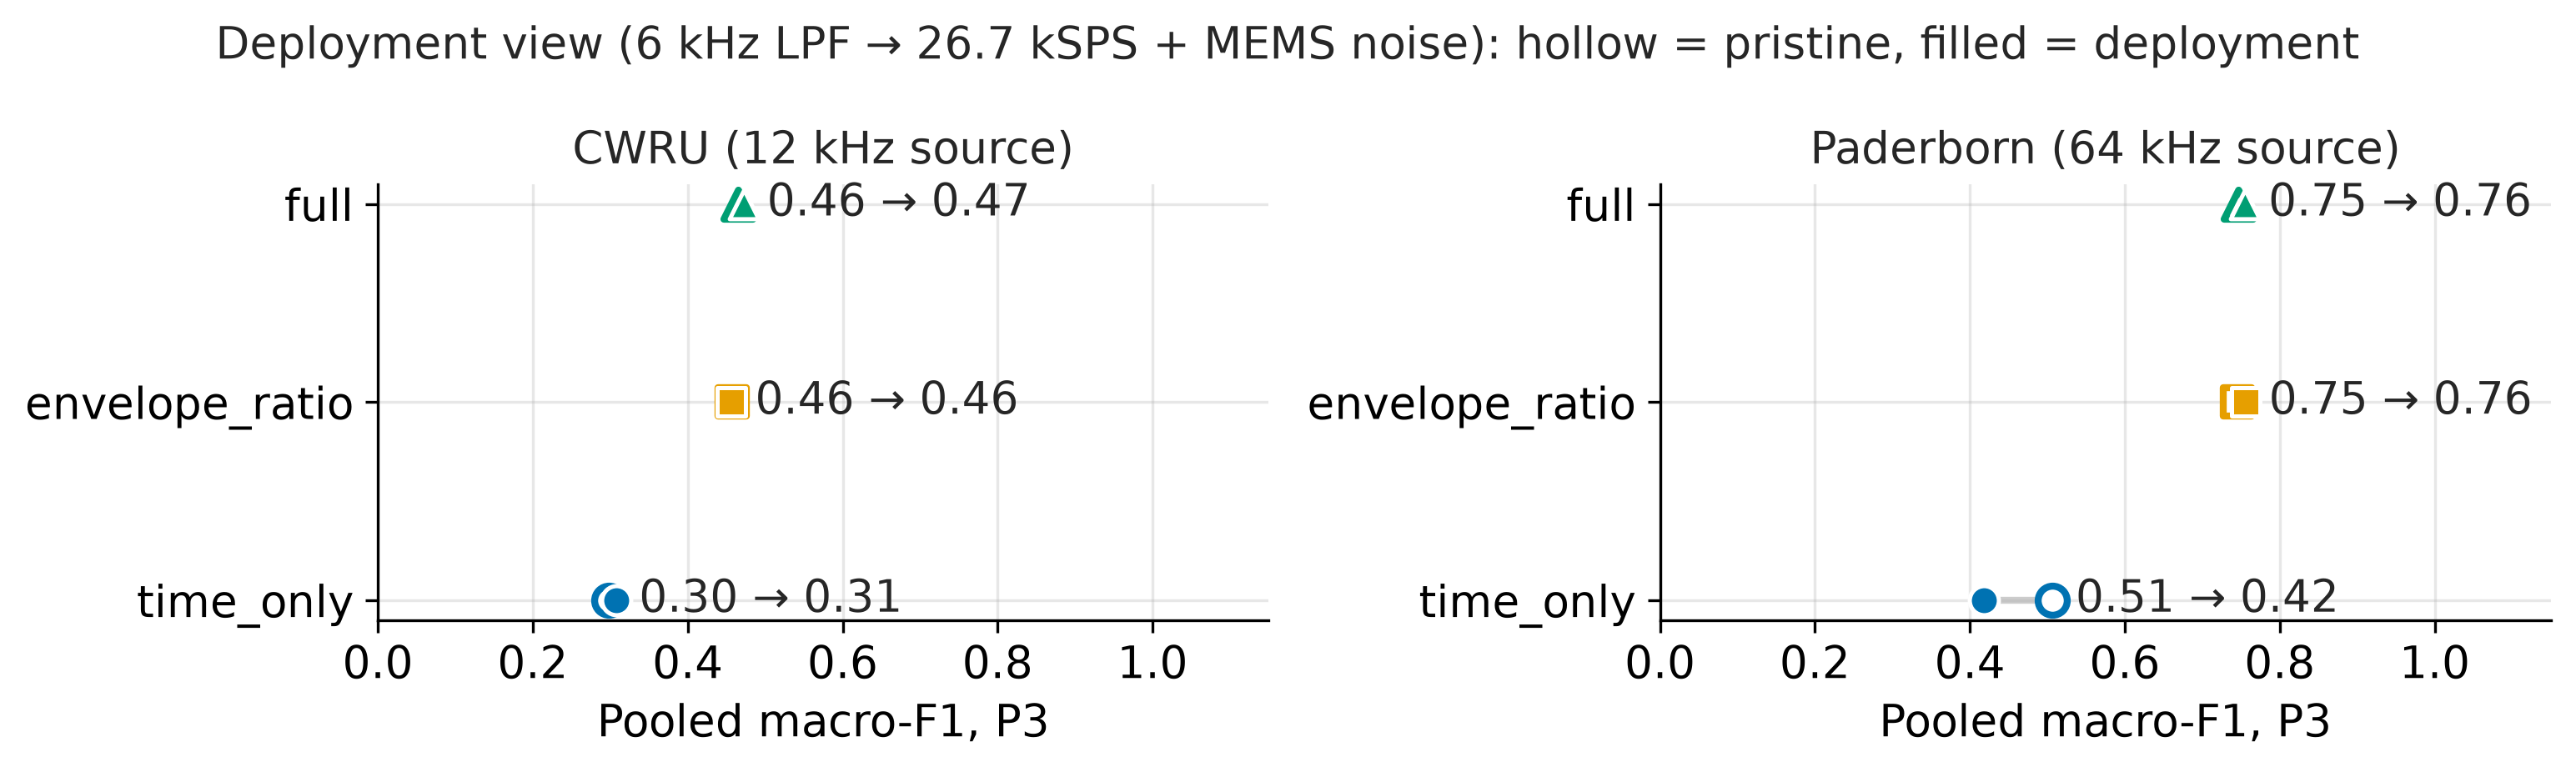
\includegraphics[width=0.85\textwidth]{figures/deployment_degradation_real.png}}
\caption{Pooled macro-F1 on P3 before (hollow) and after (filled) the simulated deployment sensor, for CWRU (left)
and Paderborn (right).}
\label{fig:deploy}
\end{figure*}

\begin{table}[t]
\caption{Cost per feature set: features, feature-vector bytes (float32), parameters (model plus standardisation) and host extraction time per 4 s window (laptop CPU, relative only).}
\label{tab:cost}
\centering
\setlength{\tabcolsep}{3pt}
\begin{tabular}{lrrrrr}
\hline
Set & Feat. & Bytes & LR par. & GBDT par. & ms \\
\hline
time\_only & 17 & 68 & 106 & 10,320 & 1.17 \\
envelope\_ratio & 39 & 156 & 238 & 5,372 & 3.66 \\
full & 40 & 160 & 244 & 5,380 & 4.14 \\
\hline
\end{tabular}
\end{table}


\subsection{Edge gateway (Orange Pi 5 Plus)}

We target a common factory layout: wired sensors stream raw vibration to one edge gateway that classifies for
all of them. The gateway is an Orange Pi 5 Plus (Rockchip RK3588), with four low-power Cortex-A55 and four
Cortex-A76 cores. \ifgateway
Table~\ref{tab:gateway} gives the measured timing. The Python pipeline takes \val{gw-env-py1}~ms per 4~s window on
one core and \val{gw-time-py1}~ms for time\_only. With all \val{gw-cores} cores busy it processes \val{gw-env-tp}
windows/s, enough for about \val{gw-env-sensors} sensors at a 2~s hop (\val{gw-time-sensors} for time\_only).

We also timed the C++ port, verified against the Python implementation, on a single core. One Cortex-A55 core
processes a 1.37~s window in \val{gw-env-cpp-little}~ms, \val{gw-env-cpp-little-rt}$\times$ faster than real time; one
Cortex-A76 core takes \val{gw-env-cpp-big}~ms. Energy is estimated rather than measured, using a published
wall-socket measurement of the board (about 5~W idle and 15~W at full load)\scite{carmo2024}. Dividing full-load
board power by throughput gives about \val{gw-env-mj}~mJ per window, or \val{gw-env-wps}~mW per sensor at capacity.

\begin{table*}[t]
\caption{Orange Pi 5 Plus edge gateway. Python: the full pipeline per 4 s window on one core, and windows per second with every core busy; sensors served in real time at a 2 s hop (compute only). C++: the ported pipeline per 1.37 s window pinned to one Cortex-A55 (little) or Cortex-A76 (big) core. Energy: estimated, full-load board power divided by throughput.}
\label{tab:gateway}
\centering
\begin{tabular}{lrrrrrr}
\hline
Feature set & Python ms & Windows/s & Sensors & C++ A55 ms & C++ A76 ms & mJ/window (est.) \\
\hline
time\_only & 6.99 & 322 & 645 & 4.43 & 0.83 & 46.5 \\
envelope\_ratio & 18.77 & 177 & 353 & 13.74 & 3.16 & 85.0 \\
\hline
\end{tabular}
\end{table*}

\else
\todo{Gateway results pending: run \texttt{make gateway} on the board.}
\fi

\FloatBarrier
% =====================================================================================================
\section{Limitations}

The intervals are wide: CWRU has \val{cwru-ids} fault identities and Paderborn \val{pb-ids}, and CWRU P3's gain is
not significant. The envelope advantage requires measured or rated-speed-constrained speed, and on Paderborn
it requires measured speed. CWRU's single healthy bearing cannot be tested under P3. Gateway energy is estimated
from a published board figure, not measured. The sensors-served figure counts compute only, without network or
I/O. The sensor view is simulated, and Paderborn's signal units are undocumented, so its added noise is
approximate. MaFaulDa states no licence, and its cage faults are counted as outer race.

% =====================================================================================================
\section{Conclusion}

Honest evaluation changes the picture of bearing fault detection. Random-window splits on CWRU score
\val{cwru-logreg-P0-env-f1} for every feature set, whereas holding out the fault drops scores to
\val{cwru-logreg-P3-env-f1}--\val{paderborn-logreg-P3-env-f1}. On those honest splits, envelope features at the
kinematic fault frequencies outperform time-domain features. The advantage is significant on Paderborn
leave-one-bearing-out, on artificial-to-real transfer and on CWRU leave-one-severity-out, but it depends on an
accurate shaft speed. A rated-speed prior suffices on CWRU; Paderborn needs a tachometer or a better estimator.
The envelope pipeline is cheap enough for a single low-power core of an edge gateway. Future work is measured
rather than estimated energy, a microcontroller implementation for wireless sensors, and speed estimation where
the shaft line is weak.

\section*{Code and Data Availability}

All code, frozen split manifests, result files and figures are at
\url{https://github.com/AKSHAJ-SHELL/vibrometer_research}. \texttt{make reproduce} reruns every experiment from
the public datasets\scite{cwru,lessmeier2016,mafaulda,mfpt}.

\section*{AI-Use Disclosure}
\todo{To be written by the author.}

% =====================================================================================================
\begin{thebibliography}{00}
\bibitem{cwru} Case Western Reserve University Bearing Data Center, ``Bearing data,'' 2024. [Online]. Available:
\url{https://engineering.case.edu/bearingdatacenter}
\bibitem{zhang2020} S. Zhang, S. Zhang, B. Wang, and T. G. Habetler, ``Deep learning algorithms for bearing fault
diagnostics---A comprehensive review,'' \textit{IEEE Access}, vol. 8, pp. 29857--29881, 2020,
doi: 10.1109/ACCESS.2020.2972859.
\bibitem{neupane2020} D. Neupane and J. Seok, ``Bearing fault detection and diagnosis using Case Western Reserve
University dataset with deep learning approaches: A review,'' \textit{IEEE Access}, vol. 8, pp. 93155--93178, 2020,
doi: 10.1109/ACCESS.2020.2990528.
\bibitem{kapoor2023} S. Kapoor and A. Narayanan, ``Leakage and the reproducibility crisis in machine-learning-based
science,'' \textit{Patterns}, vol. 4, no. 9, Art. no. 100804, 2023, doi: 10.1016/j.patter.2023.100804.
\bibitem{smith2015} W. A. Smith and R. B. Randall, ``Rolling element bearing diagnostics using the Case Western
Reserve University data: A benchmark study,'' \textit{Mech. Syst. Signal Process.}, vols. 64--65, pp. 100--131, 2015,
doi: 10.1016/j.ymssp.2015.04.021.
\bibitem{hendriks2022} J. Hendriks, P. Dumond, and D. A. Knox, ``Towards better benchmarking using the CWRU bearing
fault dataset,'' \textit{Mech. Syst. Signal Process.}, vol. 169, Art. no. 108732, 2022,
doi: 10.1016/j.ymssp.2021.108732.
\bibitem{randall2011} R. B. Randall and J. Antoni, ``Rolling element bearing diagnostics---A tutorial,''
\textit{Mech. Syst. Signal Process.}, vol. 25, no. 2, pp. 485--520, 2011, doi: 10.1016/j.ymssp.2010.07.017.
\bibitem{lessmeier2016} C. Lessmeier, J. K. Kimotho, D. Zimmer, and W. Sextro, ``Condition monitoring of bearing
damage in electromechanical drive systems by using motor current signals of electric motors: A benchmark data set
for data-driven classification,'' in \textit{Proc. Eur. Conf. PHM Soc.}, vol. 3, no. 1, 2016,
doi: 10.36001/phme.2016.v3i1.1577.
\bibitem{antoni2006} J. Antoni, ``The spectral kurtosis: A useful tool for characterising non-stationary
signals,'' \textit{Mech. Syst. Signal Process.}, vol. 20, no. 2, pp. 282--307, 2006, doi: 10.1016/j.ymssp.2004.09.001.
\bibitem{mafaulda} Federal University of Rio de Janeiro (UFRJ), ``MaFaulDa: Machinery fault database,'' 2016.
[Online]. Available: \url{http://www02.smt.ufrj.br/~offshore/mfs/page_01.html}
\bibitem{mfpt} Society for Machinery Failure Prevention Technology, ``MFPT bearing fault data sets,'' mirror, 2025.
[Online]. Available: \url{https://www.kaggle.com/datasets/emperorpein/mfpt-fault-datasets}
\bibitem{carmo2024} R. Carmo, ``A review of the Orange Pi 5+,'' \textit{Tao of Mac}, Jan. 2024. [Online]. Available:
\url{https://taoofmac.com/space/blog/2024/01/20/1800}
\end{thebibliography}

\end{document}
